\documentclass{report}
\usepackage{german}
\usepackage[utf8]{inputenc}
\usepackage{a4wide}
\usepackage{epsfig}
\usepackage{amssymb}
\usepackage{fleqn}
\usepackage[fleqn]{amsmath}
\usepackage{amsmath}
\usepackage{enumerate}
\usepackage{fancyvrb}
\usepackage{alltt}
\usepackage{epic}
\usepackage{xfrac}
\usepackage{color} 
\usepackage{theorem}
\usepackage{hyperref}
\usepackage{inconsolata}
\usepackage[all]{hypcap}
\hypersetup{
        colorlinks = true, % comment this to make xdvi work
        linkcolor  = blue,
        citecolor  = red,
        filecolor  = [rgb]{0.1, 0.1, 1.0},
        urlcolor   = [rgb]{0.1, 0.1, 1.0},
        pdfborder  = {0 0 0} 
}

\usepackage{fancyhdr}
\usepackage{lastpage} 

\pagestyle{fancy}

\renewcommand*{\familydefault}{\sfdefault}

\renewcommand{\chaptermark}[1]{\markboth{\chaptername \ \thechapter.\ #1}{}}
\renewcommand{\sectionmark}[1]{\markright{\thesection. \ #1}{}}
\fancyhead[R]{\leftmark}
\fancyhead[L]{\rightmark}

\definecolor{amethyst}{rgb}{0.2, 0.4, 0.6}
\definecolor{orange}{rgb}{1, 0.9, 0.0}

\usepackage[german]{babel}
\usepackage{babelbib}
\bibliographystyle{babunsrt}

{\theorembodyfont{\sf}
\newtheorem{Definition}{Definition}
\newtheorem{Axiom}[Definition]{Axiom}
\newtheorem{Notation}[Definition]{Notation}
\newtheorem{Korollar}[Definition]{Korollar}
\newtheorem{Lemma}[Definition]{Lemma}
\newtheorem{Satz}[Definition]{Satz}
\newtheorem{Theorem}[Definition]{Theorem}
}

\newcommand{\proof}{\vspace*{0.2cm}

\noindent
\textbf{Beweis}: }

\newcommand{\hint}{\vspace*{0.2cm}

\noindent
\textbf{Hinweis}: }
 
\newcommand{\qed}{\hspace*{\fill} $\Box$
\vspace*{0.2cm}

}

\newcommand{\eod}{\hspace*{\fill} $\diamond$}

\newcommand{\eox}{\hspace*{\fill} $\diamond$}

\newcommand{\edx}{\hspace*{\fill} $\diamond$}

% set the monospace-font to Inconsalata-g


\newcommand{\solution}{\vspace*{0.2cm}

\noindent
\textbf{L\"osung}: }

\newcounter{aufgabe}
\newcommand{\exercise}{\vspace*{0.2cm}
\stepcounter{aufgabe}

\noindent
\textbf{Aufgabe \arabic{aufgabe}}: }

\newcommand{\exercises}{\vspace*{0.2cm}
\stepcounter{aufgabe}

\noindent
\textbf{Aufgabe \arabic{aufgabe}$^*$}: }

\newcommand{\example}{\vspace*{0.2cm}

\noindent
\textbf{Beispiel}: \ }

\newcommand{\examples}{\vspace*{0.2cm}

\noindent
\textbf{Beispiele}: \ }
 
\newcommand{\remark}{\vspace*{0.2cm}
\noindent
\textbf{Bemerkung}: }

\newcommand{\lb}{\hspace*{\fill} \linebreak}

\newcommand{\ds}{\displaystyle}
\newcommand{\bruch}[2]{\displaystyle\frac{\;\displaystyle#1\;}{\;\displaystyle#2\;}}
\newcommand{\bruchs}[2]{\textstyle\frac{\;\textstyle#1\;}{\;\textstyle#2\;}}
\newcommand{\folge}[1]{\bigl(#1\bigr)_{n\in\mathbb{N}}}
\newcommand{\folgea}[1]{\bigl(#1\bigr)_{n\in\mathbb{N}}}
\newcommand{\Folge}[1]{\left(#1\right)_{n\in\mathbb{N}}}
\newcommand{\Reihe}[1]{\left(\sum\limits_{i=1}^n #1\right)_{n\in\mathbb{N}}}
\newcommand{\bint}{\displaystyle\int}
\newcommand{\dint}[2]{\displaystyle\int_{#1}^{#2}\hspace{-0.2cm}}
\newcommand{\Oh}{\mathcal{O}}
\newcommand{\df}[1]{\displaystyle\frac{\textrm{d}#1}{\textrm{d}x}}
\newcommand{\dfo}{\displaystyle\frac{\textrm{d}\;}{\textrm{d}x}}
\newcommand{\dr}{\textrm{d}}
\newcommand{\err}[1]{\textsl{error}_n(#1)}
\newcommand{\erri}[2]{\textsl{error}^{(#2)}_n(#1)}
\newcommand{\norm}[1]{\big\|#1\bigr\|_{\infty}}

\def\pair(#1,#2){\langle #1, #2 \rangle}

\newlength{\mylength}
\setlength{\mathindent}{1.3cm}

% -------------------------------------------------------------------------------------------
%                     Angaben zur Arbeit
% -------------------------------------------------------------------------------------------

\newcommand{\titel}{Implementierung eines neuronalen Netzwerkes zur Zeichenerkennung in SetlX}
\newcommand{\untertitel}{}
\newcommand{\arbeit}{Studienarbeit}
\newcommand{\studiengang}{Angewandte Informatik}
\newcommand{\autor}{Lucas Heuser und Johannes Hill}
\newcommand{\matrikelnrlh}{9706659}
\newcommand{\matrikelnrjh}{9705747}
\newcommand{\kurs}{TINF14AI-BI}
\newcommand{\firma}{Roche Diagnostics GmbH, Mannheim}
\newcommand{\abgabe}{05. September 2016}
\newcommand{\betreuerdhbw}{k.A.}
\newcommand{\abteilung}{Scientific Information Services}
\newcommand{\betreuerfirma}{Prof. Dr. Karl Stroetmann}
\newcommand{\bearbeitungszeitraum}{05.09.2016 - 29.05.2017}

\newcommand{\jahr}{2017}			% für Angabe im Copyright-Vermerk der Titelseite

% -------------------------------------------------------------------------------------------
%                     Beginn des Dokumenteninhalts
% -------------------------------------------------------------------------------------------

\begin{document}
\setcounter{secnumdepth}{3}					% Nummerierungstiefe fürs Inhaltsverzeichnis
\setcounter{tocdepth}{1}
% -------------------------------------------------------------------------------------------
%                     Titelseite
% -------------------------------------------------------------------------------------------

%\thispagestyle{plain}
\begin{titlepage}
\enlargethispage{4.0cm}

			
\begin{flushright}

\epsfig{file=dhbw-logo.eps, scale=1.5}
\end{flushright}
	
\begin{center}

\huge{\textsc{\textbf{\titel}}}\\[1.5ex]
\Large{\textbf{\untertitel}}\\[5ex]
\LARGE{\textbf{\arbeit}}\\[2ex]
\Large{Studiengang \studiengang}\\[1ex]
\normalsize{Duale Hochschule Baden-Württemberg Mannheim}\\[5ex]
von\\[1ex] \autor \\[15ex]


\end{center}
\begin{flushleft}
\begin{tabular}{ll}
%Abgabedatum:					& \quad \abgabe \\
Bearbeitungszeitraum:			& \quad \bearbeitungszeitraum   \\ 
Matrikelnummer, Kurs: 			& \quad \matrikelnr , \kurs \\ 
Ausbildungsfirma:	 			& \quad \firma \\ 
Abteilung:						& \quad \abteilung \\
Betreuer der DHBW-Mannheim:  & \quad \betreuerfirma \\ [10ex]
\rule[-0.2cm]{6.5cm}{0.5pt} \\[2ex]
\textsc{Unterschrift des Betreuers} 

%Gutachter der Dualen Hochschule: & \quad \betreuerdhbw \\ [5ex]

\end{tabular} 
\end{flushleft}
\end{titlepage} 				% erzeugt die Titelseite
\pagenumbering{Roman}						% große, römische Seitenzahlen für Titelei
\chapter*{Eidesstattliche Erklärung}

Hiermit erklären wir, dass wir die vorliegende Arbeit mit dem Thema
\begin{quote}
\textit{\titel}% -\textit{ \untertitel }
\end{quote}
selbstständig und ohne Benutzung anderer als der angegebenen Quellen und Hilfsmittel angefertigt haben. \\[2ex]
Alle Stellen, die wörtlich oder sinngemäß aus veröffentlichten und nicht veröffentlichten Schriften entnommen wurden, sind als solche kenntlich gemacht. \\[2ex]
Die Arbeit ist in gleicher oder ähnlicher Form oder auszugsweise im Rahmen einer anderen Prüfung noch nicht vorgelegt worden.
\\[10ex]


Mannheim, den \today \\[4ex]


\rule[-0.2cm]{5cm}{0.5pt} \hspace{4cm} \rule[-0.2cm]{5cm}{0.5pt} \\

\textsc{Lucas Heuser} \hspace{6,6cm} \textsc{Johannes Hill}
%\textsc{\autor} \\[10ex]

% Sperrvermerk bei Bedarf dekommentieren
%\hrule 
%\vspace*{1.0cm}
%\noindent \textbf{\Large{Sperrvermerk}}\\
%\normalsize
%Die Ergebnisse der Arbeit stehen ausschließlich dem auf dem Deckblatt aufgeführten Ausbildungsbetrieb zur Verfügung. 				% Einbinden der eidestattlichen Erklärung
%\chapter*{Freigabe durch das Ausbildungsunternehmen}

Diese Praxis- / Bachelorarbeit wurde durch das Ausbildungsunternehmen inhaltlich geprüft und zur Vorlage an der DHBW Mannheim, Studiengang Angewandte Informatik freigegeben.
\\[10ex]

Mannheim, den \today \\[4ex]


\rule[-0.2cm]{5cm}{0.5pt} \\

\textsc{\betreuerfirma} \\[10ex]
					% Einbinden der Freigabe durch das Ausbildungsunternehmen
\include{Inhalt/abstract}   				% Einbinden des Abstracts

%\maketitle
\tableofcontents
\listoffigures
%\listoftables

%\makenomenclature							% Abkürzungsverzeichnis erstellen
%
% alle Abkürzungen, die in der Bachelorarbeit verwendet werden
\nomenclature{AACR 2}{Anglo-American Cataloguing Rules 2nd edition}
\nomenclature{ACID}{Atomicity, Consistency, Isolation, Durability}
\nomenclature{Base}{Basically Available, Soft state, Eventual consistency}
\nomenclature{CQL}{Contextual Query Language}
\nomenclature{DB}{Datenbank}
\nomenclature{DBMS}{Datenbankmanagementsystem}
\nomenclature{DBS}{Datenbanksystem}
\nomenclature{DHBW}{Duale Hochschule Baden-Württemberg}
\nomenclature{DOI}{Digital Object Identifier}
\nomenclature{HTTP}{Hypertext Transfer Protocol}
\nomenclature{ISBD}{International Standard Bibliographic Description}
\nomenclature{LCC}{Library of Congress Classification}
\nomenclature{LCSH}{Library of Congress Subject Headings}
\nomenclature{LDAP}{Lightweight Directory Access Protocol}
\nomenclature{MARC}{Machine-Readable Cataloging}
\nomenclature{MVCC}{Multiversion Concurrency Control}
\nomenclature{NoSQL}{Not only SQL}
\nomenclature{OCR}{Optical Character Recognition}
\nomenclature{Org}{Organisation}
\nomenclature{PDF}{Portable Document Format}
\nomenclature{PMM}{Project Management Methodology}
\nomenclature{RDBS}{Relationales Datenbanksystem}
\nomenclature{RDG}{Roche Diagnostics GmbH}
\nomenclature{RTF}{Rich-Text Format}
\nomenclature{RTYPE}{Record Type}
\nomenclature{Sem}{Semester}
\nomenclature{SFX}{Linkresolver der Firma Ex Libris Group}
\nomenclature{SIS}{Scientific Information Services}
\nomenclature{SOAP}{Simple Object Access Protocol}
\nomenclature{SRU}{Search and Retrieve via URL}
\nomenclature{SUTRS}{Simple Unstructured Text Record Syntax}
\nomenclature{URL}{Uniform Resource Locator}
\nomenclature{USMARC}{US Machine-Readable Cataloging}
\nomenclature{W3C}{World Wide Web Consortium}
\nomenclature{XML}{Extensible Markup Language}




\pagebreak

% --------------------------------------------------------------------------------------------
%                    Inhalt der Bachelorarbeit
%---------------------------------------------------------------------------------------------  
\pagenumbering{arabic}						% arabische Seitenzahlen für den Hauptteil	
\setcounter{tocdepth}{1}

\fancyfoot[C]{--- \thepage/\pageref{LastPage}\ ---}

\fancypagestyle{plain}{%
\fancyhf{}
\fancyfoot[C]{--- \thepage/\pageref{LastPage}\ ---}
\renewcommand{\headrulewidth}{0pt}
}

\chapter{Einleitung}

\section{Ziel der Arbeit}
Diese Arbeit wurde im Rahmen einer Studienarbeit an der Dualen Hochschule Baden-Württemberg unter der Leitung von Prof. Dr. Karl Stroetmann angefertigt. Die Arbeit dient zur Unterstützung und Erweiterung der von Herrn Stroetmann gehaltenen Vorlesung \glqq Artificial-Intelligence\grqq \cite{stroetmann:2017}. Ziel der Arbeit ist es, die Vorlesung um ein praktisches Beispiel für Neuronale Netze zu erweitern. In den Vorlesungen von Herrn Stroetmann wird zur Veranschaulichung von Algorithmen und Methoden die, an mathematische Formulierungen angelehnte, Programmiersprache SetlX verwendet \cite{setlx:2017}. In dieser Programmiersprache sollte auch das Neuronale Netzwerk programmiert werden. \\
Als Basis des in dieser Studienarbeit implementierten Netzwerkes dient die Python Implementierung einer Zeichenerkennung von Michael Nielsen \cite{nielson:2017}.

\section{Aufgabe des neuronalen Netzwerks}
Ziel des in dieser Arbeit implementierten neuronalen Netzwerks ist es, handgeschriebene Zeichen zu erkennen und auszuwerten. Die eingelesenen Zeichen bestehen aus 28x28 Pixeln, welche in verschiedenen Graustufen dargestellt werden. Die Ziffern bestehen aus Werten zwischen 0 und 9. 
\begin{figure}[hbt]
	\centering
	
\includegraphics[scale=0.6]{Bilder/handdrawn_digit}
	\caption{Handgeschriebene Ziffer 5 \cite{nielson:2017}} 
	\label{fig:handwritten_digit_5} 
\end{figure}
Abb. \ref{fig:handwritten_digit_5} zeigt ein Beispiel einer solchen Ziffer. Mit Hilfe des menschlichen Auges und Gehirns ist es für die meisten Menschen ohne Probleme möglich, zu erkennen, dass es sich hierbei um eine Ziffer mit dem Wert \glqq 5\grqq handelt. Eine Erkennung mittels herkömmlicher Computeralgorithmen hingegen stellt sich allerdings als sehr komplex und schwierig heraus. Gründe hierfür sind, dass beispielsweise verschiedene Ziffern durch unterschiedliche Handschriften signifikante Unterschiede aufweisen. Auch können beim Schreibvorgang einzelne Linien durch den Druck des Stiftes schwächer oder gar nicht abgebildet werden, was die gezeichnete Zahl ebenso variieren lässt. Diese und viele weitere Faktoren führen dazu, dass eine solche Zeichenerkennung mit Hilfe von einfachen Auswertealgorithmen zu hohen Fehlerraten führt und sehr aufwendig zu implementieren ist. \\ \\
Mit Hilfe eines neuronalen Netzwerks ist es bei solch einem Problem möglich, das Netzwerk automatisch mit Hilfe von Traningsdaten zu trainieren. Das bedeutet, dem Netzwerk wird eine möglichst große Menge an Testdaten übergeben und das Netzwerk lernt automatisch mit Hilfe dieser Daten, um das Problem mit möglichst geringer Fehlerrate zu lösen. Um dies bewerkstelligen zu können, müssen die Trainingsdaten aus folgenden Komponenten bestehen:
\begin{enumerate}
\item Eingabedaten (hier: Pixel des auszuwertenden Zeichens)
\item Erwartetes Ergebnis zu jeder Eingabe (hier: 5)
\end{enumerate}

\section{Verfügbarkeit des Programmcodes auf GitHub}
Der in dieser Studienarbeit entwickelte Programmcode, sowie sämtliche Dokumentation sind in GitHub unter folgender Adresse zu finden:
\\[0.2cm]
\hspace*{1.3cm}
\href{https://github.com/lucash94/Neural-Network-in-SetlX/}{https://github.com/lucash94/Neural-Network-in-SetlX}.
\\[0.2cm]
Im Verzeichnis \glqq Studienarbeit\grqq befindet sich diese Arbeit und das Verzeichnis \glqq setlx\grqq beinhaltet die eigentliche Implementierung in SetlX. Das dritte Verzeichnis \glqq res\grqq dient zur Aufbewahrung aller sonstigen Dateien und Aufzeichnungen der Studienarbeit.

\section{Aktuelle Relevanz von neuronalen Netzen}
Die Relevanz neuronaler Netzwerke nimmt im privaten Alltag immer mehr zu. Mittlerweile bieten große IT-Unternehmen Produkte für den Massengebrauch an, welche sich der Hilfe neuronaler Netzwerke bedienen. Einige populäre Beispiele des Einsatzes neuronaler Netzwerke sind:
\begin{enumerate}
\item Verbesserung der Übersetzungsergebnisse des Google Translaters wurden mittels neuronalen Netzen und einer hohen Anzahl an Trainingsdaten ermöglicht. Am 26.09.2016 wurde das Google Neural Machine Translation system (GNMT) in das Online-Tool eingeführt. \cite{gnmt:2017}
\item Das Programm AlphaGo des Unternehmens Google DeepMind ist spezialisiert auf das aus China stammende Brettspiel Go. Mit Hilfe eines neuronalen Netzes war AlphaGo das erste Computerprogramm, welches einen professionellen Go-Spieler schlagen konnte. \cite{alphago:2017}
\item Die Foto- und Videobearbeitungsapplikation Prisma nutzt ein neuronales Netzwerk um Fotos und Videos von Nutzern mit Effekten und Filtern basierend auf berühmten Kunstwerken zu versehen. \cite{prismaai:2017}
\end{enumerate}

\section{Aufbau der Arbeit}
Diese Arbeit ist in drei Kategorien unterteilt. Zu Beginn der Arbeit wird ein Überblick über das theoretische Wissen sowie den allgemeinen Aufbau und die Funktion neuronaler Netze gegeben. Anschließend wird die konkrete Umsetzung des Projektes in SetlX erläutert. Hierbei wird kurz die Beschaffung der Datensätze, gefolgt von der Hauptimplementierung, besprochen. Ebenso gibt es einen Abschnitt über ein weiteres SetlX-Programm, welches die Ausgabe des neuronalen Netzwerkes grafisch darstellt. \\
Der letzte Abschnitt der Arbeit befasst sich mit der Auswertung des Ergebnisses. Hierbei wird die Performance des finalen Programmes diskutiert sowie ein Fazit über den Erfolg oder Misserfolg der Arbeit gezogen.
\chapter{Theorie}

\section{SetlX}

\section{MNIST}

\section{Neuronales Netzwerk}
In diesem Abschnitt der Arbeit wird der Aufbau eines neuronalen Netzwerks näher betrachtet und entsprechend auf die Terminologie in diesem Bereich eingegangen. \\
Neuronale Netzwerke sind den biologischen Neuronen nachempfunden und setzen sich daher aus Vielzahl von Neuronen zusammen. Darüber hinaus ist ein Netzwerk in mehrere Schichten untergliedert (siehe Abb.\ref{fig:neural_network_extended}). So wird die erste Schicht auf der linken Seite auch als \textit{Eingabeschicht} und alle korrespondierenden Eingabeknoten als Eingabeneuron bezeichnet. Die letzte Schicht, die sogenannte \textit{Ausgabeschicht}, beinhaltet dagegen alle \textit{Ausgabeneuronen}. Alle Schichten zwischen der Eingabe und der Ausgabe tragen die Bezeichnung des \textit{Hidden Layer}, wobei ein Netzwerk mehrere dieser Schichten aufweisen kann. In der folgenden Grafik ist ein 4-Layer-Netzwerk abgebildet, das zwei \textit{Hidden Layer} besitzt. Diese mehrschichtigen Netzwerke werden ebenfalls als \textit{Multilayer Perceptrons} oder \textit{MLPs} bezeichnet, obwohl das Netzwerk sich aus Sigmoid-Neuronen zusammensetzt.
\begin{figure}[hbt]
	\centering
	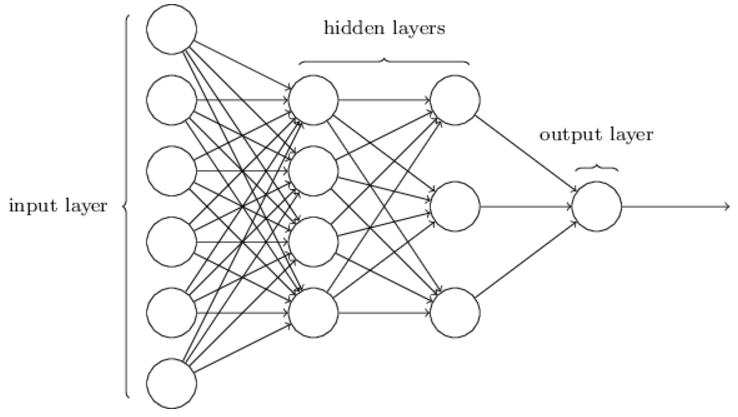
\includegraphics[scale=0.6]{Bilder/neural_network_extended}
	\caption{Aufbau des neuronalen Netzwerks hinsichtlich der einzelnen Layer.} 
	\label{fig:neural_network_extended} 
\end{figure}

\noindent
Für die Zusammensetzung von Eingabe- und Ausgabeschichten in einem Netzwerk, fällt die Betrachtung auf die Erkennung einer handgeschrieben "9". Als Eingabewerte dienen dem Netzwerk die Intensitäten der Bildpixel. Liegt ein Graustufenbild der Größe von 64x64 Pixeln vor, leiten sich daraus 4096 Eingabeknoten  mit skalierten Intensitätswerten zwischen 0 und 1 ab. Die Ausgabeschicht beinhaltet dagegen nur ein Neuron, um eine entsprechende Klassifizierung der "9" vornehmen zu können. \\[0.2cm]
\hspace*{1.3cm}
$ 
\begin{array}[t]{lcll}
	\mathtt{output} < 0.5 \quad\rightarrow\quad \mbox{"Eingabebild ist keine 9"} \\[0.2cm]
	\mathtt{output} \geq 0.5 \quad\rightarrow\quad \mbox{"Eingabebild ist eine 9"}
\end{array}
$
\\[0.2cm]
Im Vergleich hierzu ist der Aufbau der Hidden-Layer nicht durch irgendwelche Regeln ableitbar. Zum Einsatz kommen Heuristiken, die das Verhalten eines Netzwerkes bestimmen, welches ausgehend vom Experiment erwartet und gewünscht wird. Zum Beispiel kann Untersucht werden, wie die Lernrate des Netzwerks sich im Verhältnis zu der Anzahl an Hidden-Layer verhält. \\

\noindent
Bisher viel die Betrachtung in dieser Arbeit auf neuronale Netze, bei denen die Ausgabe einer Schicht die Eingabe in der nächsten Schicht darstellte. Solche Netzwerke werden auch \textit{Feedforward Neural Networks} bezeichnet. Hierunter ist das das nicht Auftreten von Schleifen zu verstehen - sprich, Informationen werden im Netzwerk immer von Layer $n$ zu Layer $n+1$ übergeben. Somit kann verhindert werden, dass das Netzwerk in gewissen Fällen bei der Eingabe der Sigmoid-Funktion $\sigma$ von dessen Ausgabe abhängig ist. \\
Ebenfalls gibt es Netzwerke bei denen sogenannte \textit{Feedback Loops} möglich sind. In diesem Fall handelt es sich um \textit{Recurrent Neural Networks}. Die Idee hinter diesem Modell ist, dass bestimmte Neuronen über einen definierten Zeitraum aktiv sind bevor sie inaktiv werden. Dies kann andere Neuronen anregen, ebenfalls über einen gewissen Zeitraum aktiv zu sein und eine entsprechende Kettenreaktion auslösen (Kaskade). Schleifen stellen in diesem Modell kein Problem dar, da die Ausgabe eines Neurons erst zu einem späteren Zeitpunkt die Eingabe beeinflusst. \\
Stellt man diese Arten von neuronalen Netzwerken gegenüber, so lässt sie zum heutigen Zeitpunkt die Aussage treffen, dass Feedback Neural Networks weniger Verbreitung finden. Dies ist begründet in der Leistungsfähigkeit der Lernalgorithmen. Jedoch sollte an dieser Stelle berücksichtigt werden, dass mittels Feedback Neural Networks bestimmte Probleme mit einem geringeren architektonischen Aufwand gelöst werden können. Darüber hinaus bildet der komplexere logische Aufbau eines solchen Netzwerks, das menschliche Verhalten besser ab.

\section{Perceptrons}
Ein Perceptron ist ein mathematisches Modell zur Abbildung eines künstliches Neurons in einem Netzwerk. Es wird für die Entscheidungsfindung herangezogen, indem verschiedene Aussagen abgewägt werden. Hierbei nimmt das Perceptron eine Menge von Eingaben $x_n$ mit $n \in \{1, \cdots, m\}$ und berechnet einen einzigen binären Ausgabewert (siehe Abb. \ref{fig:perceptron}). 
\begin{figure}[hbt]
	\centering
	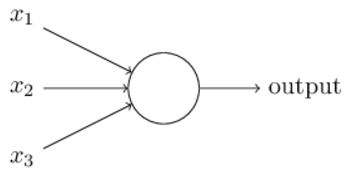
\includegraphics[scale=0.6]{Bilder/perceptron}
	\caption{Percetron mit den Eingaben $x_1, x_2, x_3$ und der Ausgabe $\mathtt{output}$.} 
	\label{fig:perceptron} 
\end{figure}

\noindent
Für jeden Eingabewert $x_n$ wird eine Gewichtung $w_n$ mit $n \in \{1, \cdots, m\}$ zugeordnet. Der Ausgabewerte $\mathtt{output}$ wird mittels der gewichteten Summe $\sum_j w_j x_k$ und einem definierten Grenzwert $\mathtt{threshold}$ bestimmt.
\begin{equation}
	\mathtt{output} := \left\{
	\begin{array}{ll}
 		0 & \displaystyle \mbox{falls}\quad \sum\limits_j w_j x_j \leq \mathtt{threshold} \\[0.5cm]
 		1 & \displaystyle \mbox{falls}\quad \sum\limits_j w_j x_j > \mathtt{threshold}
	\end{array}\right.
\end{equation}

\noindent
Der Aufbau des Netzwerks leitet sich aus den unterschiedlichen Modellen der Entscheidungsfindung ab und wird mit Hilfe der Perceptrons abgebildet (siehe Abb. \ref{fig:perceptron_models}).
\begin{figure}[hbt]
	\centering
	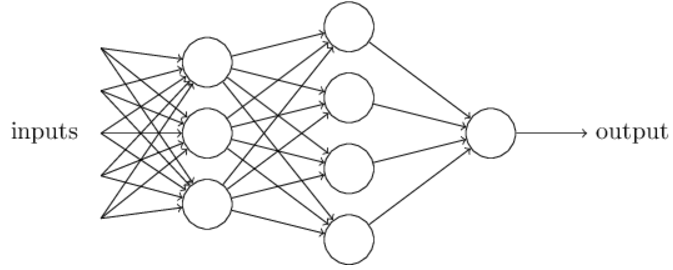
\includegraphics[scale=0.75]{Bilder/perceptron_models}
	\caption{Unterschiedliche Möglichkeiten der Entscheidungsfindung.} 
	\label{fig:perceptron_models} 
\end{figure}
Eine Entscheidungsmöglichkeit wird hierbei durch das Perceptron dargestellt. Weiterhin wird eine Spalte von Perceptrons als \textit{Layer} bezeichnet. Der erste Layer fällt Entscheidungen auf Basis der Eingabewerte, indem er diese abwägt. Jedes Perceptron des zweiten Layers hingegen, wägt für die Entscheidungsfindung die Resultate des ersten Layers ab. Ein Perceptron auf dem zweiten Layer kann somit eine Entscheidung auf einer abstrakteren und komplexeren Ebene durchführen. Auf diese Weise kann sich ein vielschichtiges Netzwerk von Perceptrons in ein anspruchsvolles Modell zur Entscheidungsfindung entwickeln. \\

\noindent
Im folgenden wird die mathematische Beschreibung von Perceptrons vereinfacht, indem Änderungen an der Notation für $\sum_j w_j x_j > \mathtt{threshold}$ vorgenommen werden. Für die Beschreibung der Summe $\sum_j w_j x_j$ werden die Vektoren $w$ und $x$ eingeführt, wodurch sich die Schreibweise $w \cdot x \equiv \sum_j w_j x_j$ ergibt. Des Weiteren wird der $\mathtt{threshold}$ auf die andere Seite der Ungleichung gezogen und erhält die Bezeichnung \textit{Bias}, $b \equiv \mathtt{-threshold}$. 
\begin{equation}
	\mathtt{output} := \left\{
	\begin{array}{ll}
 		0 & \displaystyle \mbox{falls}\quad w \cdot x + b \leq 0 \\[0.2cm]
 		1 & \displaystyle \mbox{falls}\quad w \cdot x + b > 0
	\end{array}\right.
\end{equation}
Somit nimmt der Bias Einfluss auf die binäre Ausgabe $\mathtt{output}$, weshalb der Bias eine Ausgabe mit einem hohen positiven oder negativen Wert mit einer höheren Wahrscheinlichkeit bedingen kann. \\

\noindent
Im vorherigen Abschnitt wurden Perceptrons als ein Methode für die Entscheidungsfindung beschrieben. Ein weiterer Anwendungsfall besteht in der Berechnung von logischen Funktion wie z.B. $\mathtt{AND}$, $\mathtt{OR}$ und $\mathtt{NAND}$. Fällt die Betrachtung auf ein Perceptron mit 2 Eingaben deren Gewichtung jeweils den Wert -2 aufweisen und einen Bias von 3, so ergibt sich folgende Abbildung (siehe Abb. \ref{fig:perceptron_example}).
\begin{figure}[hbt]
	\centering
	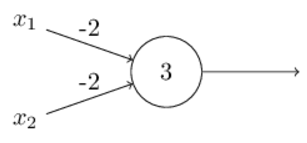
\includegraphics[scale=0.6]{Bilder/perceptron_example}
	\caption{Percetron mit zwei Eingaben -2 und einem Bias von 3.} 
	\label{fig:perceptron_example} 
\end{figure}

\noindent
Weisen die Eingaben $x_1, x_2$ den Wert 0 auf, ergibt sich für den $\mathtt{output}$ den Wert 1. Sind die Eingabewerte für $x_1, x_2$ -1 ergibt sich für den $\mathtt{output}$ den Wert -1. Der Aufbau beschreibt somit einen $\mathtt{NAND}$ Gatter.\\[0.2cm]
\hspace*{1.3cm}
$
\begin{array}[t]{lcll}
	w \cdot x + b & = & \mathtt{output} \\[0.2cm]
	(-2)*0+(-2)*0+3 & = & 1 \\[0.2cm]
	(-2)*1+(-2)*1+3 & = & -1
\end{array}
$
\\[0.2cm]
$\mathtt{NAND}$ Gatter können verwendet werden, um die unterschiedlichsten Berechnungen durchzuführen. Im Folgenden fällt die Betrachtung auf die Addition von zwei Bits $x_1$ und $x_2$. Für die Berechnung wird die bitweise Summe $x_1 \oplus x_2$ gebildet, wobei ein $\mathtt{carry bit}$ den Wert 1 annimmt, sobald $x_1$ und $x_2$ gleich 1.
\begin{figure}[hbt]
	\centering
	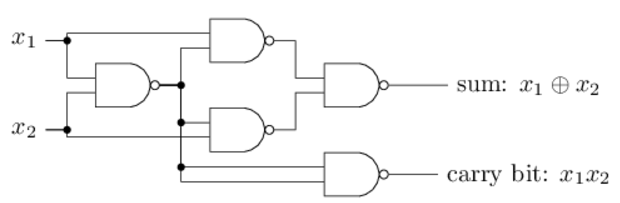
\includegraphics[scale=0.6]{Bilder/nand_gatter}
	\caption{$\mathtt{NAND}$ Gatter mit den Eingaben $x_1$ und $x_2$.} 
	\label{fig:nand_gatter} 
\end{figure}

\noindent
Um ein gleichwertiges Netzwerk abzuleiten, werden die $\mathtt{NAND}$ Gatter durch Perceptrons mit jeweils 2 Eingaben ersetzt. Hierbei weisen die Gewichtungen $w_1, w_2$ den Wert -2 und der Bias $b$ den Wert 3 auf. 
\begin{figure}[hbt]
	\centering
	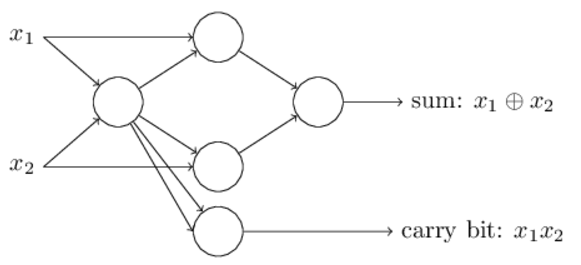
\includegraphics[scale=0.6]{Bilder/nand_gatter_perceptron}
	\caption{$\mathtt{NAND}$ Gatter Aufbau mit Perceptrons.} 
	\label{fig:nand_gatter_perceptron} 
\end{figure}

\noindent
In einem weiteren Schritt wird die Abbildung eines $\mathtt{NAND}$ Gatter mit Perceptrons vereinfacht. Dazu werden mehrere Eingänge eines Perceptrons zu einem zusammengefasst, weshalb aus den zwei Eingaben -2 der Wert -4 resultiert. Ebenfalls werden die Eingaben in einem sogenannten \textit{Input Layer} zusammengefasst, wobei durch die Notation eine Eingabe nicht mit einem Perceptron gleichzustellen ist.
\begin{figure}[hbt]
	\centering
	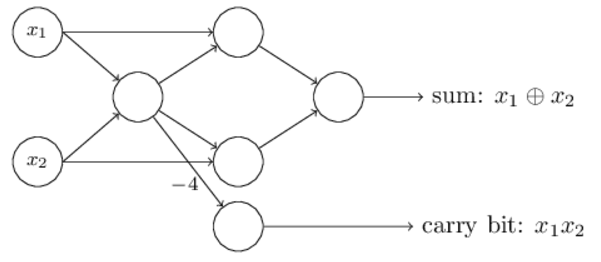
\includegraphics[scale=0.6]{Bilder/nand_gatter_perceptron_simplified}
	\caption{Vereinfachter $\mathtt{NAND}$ Gatter Aufbau mit Perceptrons.} 
	\label{fig:nand_gatter_perceptron_simplified} 
\end{figure}

\noindent
Dieser Anwendungsfall zeigt, dass mit Perceptrons unterschiedliche Berechnungen durchgeführt werden können. Implementierte Lernalgorithmen können Gewichtungen sowie den Bias automatisch durch entsprechende Stimuli im Netzwerk anpassen und ermöglichen die Nutzung von künstliche Neuronen, die sich von herkömmlichen Logik Gattern unterscheiden. Neuronale Netze können somit über einen definierten Zeitraum lernen, wie bestimmte Probleme zu lösen sind. 

\section{Sigmoid Neurons}
Für die Entwicklung lernender Algorithmen in einem Netzwerk mit Perceptrons, fällt unsere Betrachtung auf das Beispiel der Erkennung von handgeschriebenen Zahlen. Die Eingabe für das Netzwerk könnten die Raw Pixeldaten der eingescannten Bilder darstellen, welche die handgeschriebenen Zahlen abbilden. Das Ziel an dieser Stelle ist, dass das Netzwerk anhand der Veränderungen von \textit{Weights} und \textit{Biases} lernt eine korrekte Klassifizierung der Zahlen vorzunehmen. \\
Das Modifizieren der \textit{Weights} und \textit{Biases} kann das Verhalten des Netzwerkes und deren Entscheidungsfindung zu Problemen beeinflussen. Angenommen die Erkennung und Klassifizierung einer Zahl wurde durch das Netzwerk falsch vorgenommen, so können durch kleine Veränderungen an den \textit{Weights} und \textit{Biases} eine Korrektur durchgeführt werden. Dieses stetige Modifizieren der Werte über einen definierten Zeitraum ermöglicht ein lernendes Netzwerk (siehe Abb. \ref{fig:sigmoid_learning}). 
\begin{figure}[hbt]
	\centering
	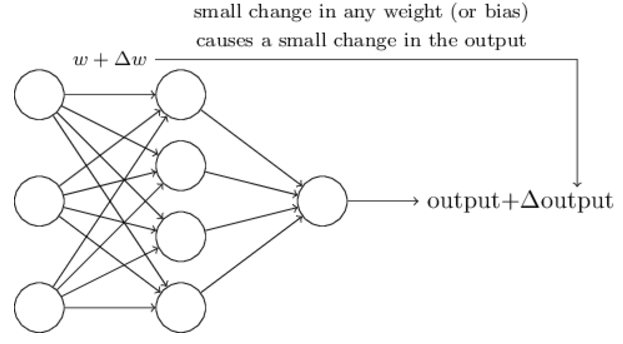
\includegraphics[scale=0.7]{Bilder/sigmoid_learning}
	\caption{Modifizieren von Weights und Biases schaffen lernendes Netzwerk.} 
	\label{fig:sigmoid_learning} 
\end{figure}

\noindent
Dieses wünschenswerte Verhalten eines lernenden Netzwerks kann durch Perceptrons nicht gewährleistet werden, da eine Veränderung der Weights und Biases den Ausgabewerte $\mathtt{output}$ eines Neurons umkehren kann. Dadurch kann das komplette Verhalten zur Klassifizierung von Zahlen beeinflusst werden, wobei zuvor falsch erkannte Zahlen nun richtig klassifiziert werden und umgekehrt. Mit Hilfe der Einführung des Sigmoid Neurons soll dieser Fehler behoben werden. Eine Änderung der Weights und Biases bei diesem künstlichen Neuron soll nur marginale Änderungen an dem Ausgabewert $\mathtt{output}$ vornehmen. Diese Erweiterung des Neurons begünstigt ein Netzwerk selbständig die Klassifizierung von Zahlen zu optimieren. \\

\noindent
Der Aufbau des Sigmoid Neurons ähnelt dem Perceptron, wobei das Neuron eine Anzahl von Eingabewerten $x_n$ mit $n \in \{1, \cdots ,m\}$ entgegennimmt und ausgehend von diesen Informationen den $\mathtt{output}$ ermittelt. Der wesentliche Unterschied zwischen diesen zwei Typen von Neuronen liegt in dem Wertebereich des $\mathtt{output}$. Bei dem Sigmoid Neuron kann dieser alle Werte zwischen 0 und 1 annehmen, sprich $\mathtt{output} \in [0 .. 1]$. Weiterhin weist auch diese Art von Neuronen für jeden Eingabewert eine Gewichtung $w_n$ mit $n \in \{1 .. n\}$ sowie einen Bias auf. \\
Für die Berechnung des $\mathtt{output}$ wird in diesem Kontext die \textit{Sigmoid Funktion} $\sigma(z)$ angewendet.
\begin{equation}
	\sigma(z) \equiv \frac{1}{1+e^{-z}} \quad\mbox{mit}\quad z = w \cdot x + b
\end{equation}
Unter Berücksichtigung der Eingabewerte $x_n$ mit $n \in \{1 .. n\}$ und der Weights  $w_n$ mit $n \in \{1 .. n\}$ ergibt sich die folgende Formel:
\begin{equation}
	\sigma(z) \equiv \frac{1}{1+\exp(-\sum_j w_j x_j - b)}
\end{equation}
Dabei weist das Sigmoid Neuron weiterhin das gleiche Verhalten wie ein Perceptron auf, wenn eine Grenzwertbetrachtung durchführt wird. \\[0.2cm]
\hspace*{1.3cm}
$
\begin{array}[t]{lcll}
	\lim\limits_{z \to \infty}{\sigma(z)} \approx 1 \quad\quad bzw. \\[0.2cm]
	\lim\limits_{z \to -\infty}{ \sigma(z)} \approx 0
\end{array}
$
\\[0.2cm]
Dieses Verhalten wird weiterhin verdeutlicht, wenn die Betrachtung auf den folgenden Funktionsgraph fällt (siehe Abb. \ref{fig:sigmoid_plot}). Für große $z$ nimmt die Funktion den Wert 1 an und für kleine $z$ nimmt die Funktion den Wert 0 an.
\begin{figure}[hbt]
	\centering
	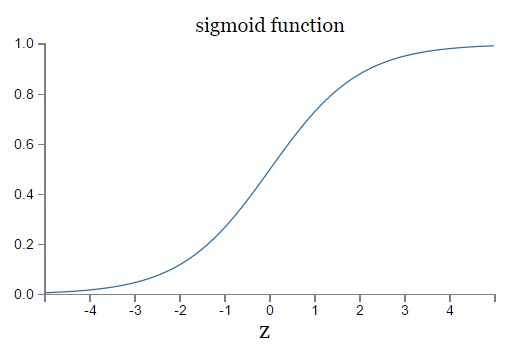
\includegraphics[scale=0.6]{Bilder/sigmoid_plot}
	\caption{Sigmoid Funktion $\sigma(z)$.} 
	\label{fig:sigmoid_plot} 
\end{figure}

\noindent
Im Vergleich hierzu die Stufenfunktion, die das Verhalten eines Perceptrons abbildet (siehe Abb. \ref{fig:perceptron_plot}).
\begin{figure}[hbt]
	\centering
	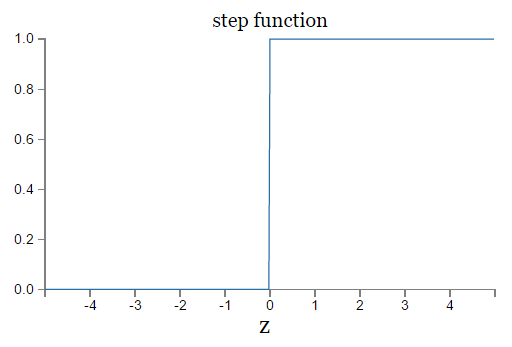
\includegraphics[scale=0.6]{Bilder/perceptron_plot}
	\caption{Sigmoid Funktion $\sigma(z)$.} 
	\label{fig:perceptron_plot} 
\end{figure}
Die Vorteile der Sigmoid Funktion liegen in den marginalen Änderungen $\delta w_j$ bei den Gewichtungen und $\delta b$ im Bias, welche eine marginale Änderung am $\delta\mathtt{output}$ vornehmen. Damit stellt $\delta\mathtt{output}$ die lineare Funktion bezüglich der Änderungen  $\delta w_j$ und $\delta b$ in den Weights und Bias dar.
\begin{equation}
	\Delta\mathtt{output} \equiv \sum_{j}{\frac{\partial\mathtt{output}}{\partial w_j}\Delta w_j+\frac{\partial\mathtt{output}}{\partial b}\Delta b_j}
\end{equation}
Diese Linearität begünstigt die Wahl von kleinen Änderungen in den Weights und Biases, um das Verhalten für ein lernendes Netzwerk abzuleiten.   

\section{Netzwerk zur Klassifizierung von handgeschrieben Zahlen}
%\chapter{Theorie}

\section{Neuronales Netzwerk}
In diesem Abschnitt der Arbeit wird der Aufbau eines neuronalen Netzwerks näher betrachtet und entsprechend auf die Terminologie in diesem Bereich eingegangen. \\
Neuronale Netzwerke sind den biologischen Neuronen nachempfunden und setzen sich daher aus Vielzahl von Neuronen zusammen. Darüber hinaus ist ein Netzwerk in mehrere Schichten untergliedert (siehe Abb.\ref{fig:neural_network_extended}). So wird die erste Schicht auf der linken Seite auch als \textit{Eingabeschicht} und alle korrespondierenden Eingabeknoten als Eingabeneuron bezeichnet. Die letzte Schicht, die sogenannte \textit{Ausgabeschicht}, beinhaltet dagegen alle \textit{Ausgabeneuronen}. Alle Schichten zwischen der Eingabe und der Ausgabe tragen die Bezeichnung des \textit{Hidden Layer}, wobei ein Netzwerk mehrere dieser Schichten aufweisen kann. In der folgenden Grafik ist ein 4-Layer-Netzwerk abgebildet, das zwei \textit{Hidden Layer} besitzt. Diese mehrschichtigen Netzwerke werden ebenfalls als \textit{Multilayer Perceptrons} oder \textit{MLPs} bezeichnet, obwohl das Netzwerk sich aus Sigmoid-Neuronen zusammensetzt.
\begin{figure}[hbt]
	\centering
	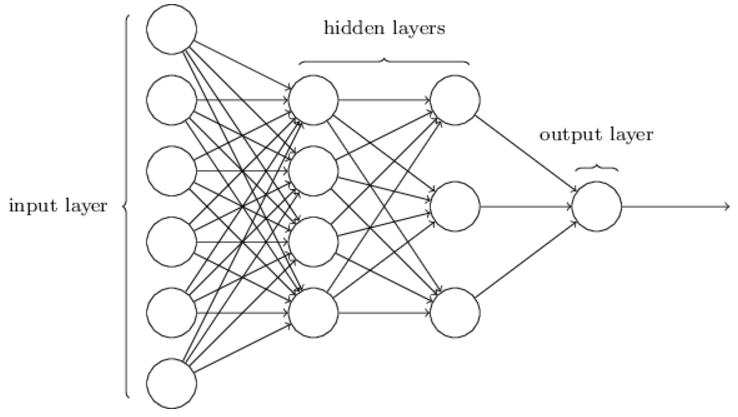
\includegraphics[scale=0.6]{Bilder/neural_network_extended}
	\caption{Aufbau des neuronalen Netzwerks hinsichtlich der einzelnen Layer.} 
	\label{fig:neural_network_extended} 
\end{figure}

\noindent
Für die Zusammensetzung von Eingabe- und Ausgabeschichten in einem Netzwerk, fällt die Betrachtung auf die Erkennung einer handgeschrieben "9". Als Eingabewerte dienen dem Netzwerk die Intensitäten der Bildpixel. Liegt ein Graustufenbild der Größe von 64x64 Pixeln vor, leiten sich daraus 4096 Eingabeknoten  mit skalierten Intensitätswerten zwischen 0 und 1 ab. Die Ausgabeschicht beinhaltet dagegen nur ein Neuron, um eine entsprechende Klassifizierung der "9" vornehmen zu können. \\[0.2cm]
\hspace*{1.3cm}
$ 
\begin{array}[t]{lcll}
	\mathtt{output} < 0.5 \quad\rightarrow\quad \mbox{"Eingabebild ist keine 9"} \\[0.2cm]
	\mathtt{output} \geq 0.5 \quad\rightarrow\quad \mbox{"Eingabebild ist eine 9"}
\end{array}
$
\\[0.2cm]
Im Vergleich hierzu ist der Aufbau der Hidden-Layer nicht durch irgendwelche Regeln ableitbar. Zum Einsatz kommen Heuristiken, die das Verhalten eines Netzwerkes bestimmen, welches ausgehend vom Experiment erwartet und gewünscht wird. Zum Beispiel kann untersucht werden, wie die Lernrate des Netzwerks sich im Verhältnis zu der Anzahl an Hidden-Layer verhält. \\

\noindent
Bisher fiel die Betrachtung in dieser Arbeit auf neuronale Netze, bei denen die Ausgabe einer Schicht die Eingabe in der nächsten Schicht darstellte. Solche Netzwerke werden auch \textit{Feedforward Neural Networks} bezeichnet. Hierunter ist das nicht Auftreten von Schleifen zu verstehen - sprich, Informationen werden im Netzwerk immer von Layer $n$ zu Layer $n+1$ übergeben. Somit kann verhindert werden, dass das Netzwerk in gewissen Fällen bei der Eingabe der Sigmoid-Funktion $\sigma$ von dessen Ausgabe abhängig ist. \\
Ebenfalls gibt es Netzwerke bei denen sogenannte \textit{Feedback Loops} möglich sind. In diesem Fall handelt es sich um \textit{Recurrent Neural Networks}. Die Idee hinter diesem Modell ist, dass bestimmte Neuronen über einen definierten Zeitraum aktiv sind bevor sie inaktiv werden. Dies kann andere Neuronen anregen, ebenfalls über einen gewissen Zeitraum aktiv zu sein und eine entsprechende Kettenreaktion auslösen (Kaskade). Schleifen stellen in diesem Modell kein Problem dar, da die Ausgabe eines Neurons erst zu einem späteren Zeitpunkt die Eingabe beeinflusst. \\
Stellt man diese Arten von neuronalen Netzwerken gegenüber, so lässt sie zum heutigen Zeitpunkt die Aussage treffen, dass Feedback Neural Networks weniger Verbreitung finden. Dies ist begründet in der Leistungsfähigkeit der Lernalgorithmen. Jedoch sollte an dieser Stelle berücksichtigt werden, dass mittels Feedback Neural Networks bestimmte Probleme mit einem geringeren architektonischen Aufwand gelöst werden können. Darüber hinaus bildet der komplexere logische Aufbau eines solchen Netzwerks das menschliche Verhalten besser ab.

\section{Perceptrons}
Ein Perceptron ist ein mathematisches Modell zur Abbildung eines künstliches Neurons in einem Netzwerk. Es wird für die Entscheidungsfindung herangezogen, indem verschiedene Aussagen abgewägt werden. Hierbei nimmt das Perceptron eine Menge von Eingaben $x_n$ mit $n \in \{1, \cdots, m\}$ und berechnet einen einzigen binären Ausgabewert (siehe Abb. \ref{fig:perceptron}). 
\begin{figure}[hbt]
	\centering
	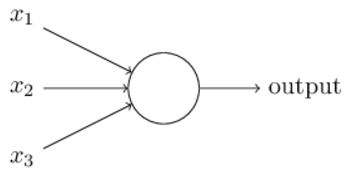
\includegraphics[scale=0.6]{Bilder/perceptron}
	\caption{Percetron mit den Eingaben $x_1, x_2, x_3$ und der Ausgabe $\mathtt{output}$.} 
	\label{fig:perceptron} 
\end{figure}

\noindent
Für jeden Eingabewert $x_n$ wird eine Gewichtung $w_n$ mit $n \in \{1, \cdots, m\}$ zugeordnet. Der Ausgabewerte $\mathtt{output}$ wird mittels der gewichteten Summe $\sum_j w_j x_k$ und einem definierten Grenzwert $\mathtt{threshold}$ bestimmt.
\begin{equation}
	\mathtt{output} := \left\{
	\begin{array}{ll}
 		0 & \displaystyle \mbox{falls}\quad \sum\limits_j w_j x_j \leq \mathtt{threshold} \\[0.5cm]
 		1 & \displaystyle \mbox{falls}\quad \sum\limits_j w_j x_j > \mathtt{threshold}
	\end{array}\right.
\end{equation}

\noindent
Der Aufbau des Netzwerks leitet sich aus den unterschiedlichen Modellen der Entscheidungsfindung ab und wird mit Hilfe der Perceptrons abgebildet (siehe Abb. \ref{fig:perceptron_models}).
\begin{figure}[hbt]
	\centering
	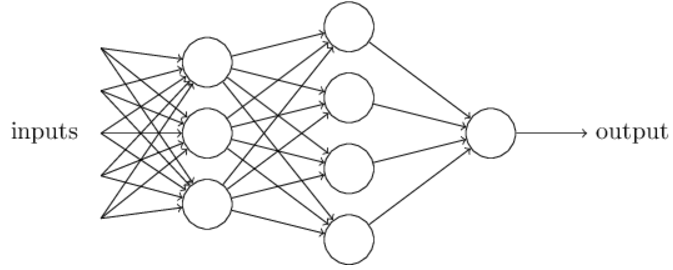
\includegraphics[scale=0.75]{Bilder/perceptron_models}
	\caption{Unterschiedliche Möglichkeiten der Entscheidungsfindung.} 
	\label{fig:perceptron_models} 
\end{figure}
Eine Entscheidungsmöglichkeit wird hierbei durch das Perceptron dargestellt. Weiterhin wird eine Spalte von Perceptrons als Schicht bezeichnet. Die erste Schicht fällt Entscheidungen auf Gewichtung der Eingabewerte, indem er diese abwägt. Jedes Perceptron der zweiten Schicht hingegen, wägt für die Entscheidungsfindung die Resultate der ersten Schicht ab. Ein Perceptron auf der zweiten Schicht kann somit eine Entscheidung auf einer abstrakteren und komplexeren Ebene durchführen. Auf diese Weise kann sich ein vielschichtiges Netzwerk von Perceptrons in ein anspruchsvolles Modell zur Entscheidungsfindung entwickeln. \\

\noindent
Im folgenden wird die mathematische Beschreibung von Perceptrons vereinfacht, indem Änderungen an der Notation für $\sum_j w_j x_j > \mathtt{threshold}$ vorgenommen werden. Für die Beschreibung der Summe $\sum_j w_j x_j$ werden die Vektoren $\mathbf{w}$ und $\mathbf{x}$ eingeführt, wodurch sich die Schreibweise $\mathbf{w} \cdot \mathbf{x} \equiv \sum_j w_j x_j$ ergibt. Des Weiteren wird der $\mathtt{threshold}$ auf die andere Seite der Ungleichung gezogen und erhält die Bezeichnung \textit{Vorbelastung}, $b \equiv \mathtt{-threshold}$. 
\begin{equation}
	\mathtt{output} := \left\{
	\begin{array}{ll}
 		0 & \displaystyle \mbox{falls}\quad \mathbf{w} \cdot \mathbf{x} + b \leq 0 \\[0.2cm]
 		1 & \displaystyle \mbox{falls}\quad \mathbf{w} \cdot \mathbf{x} + b > 0
	\end{array}\right.
\end{equation}

\noindent
Dieses mathematische Verhalten wird durch die folgende Stufenfunktion verdeutlicht (siehe Abb. \ref{fig:perceptron_plot}).
\begin{figure}[hbt]
	\centering
	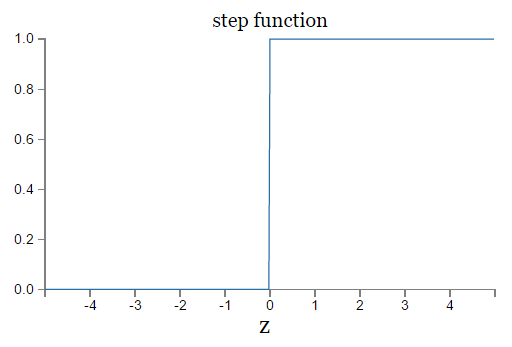
\includegraphics[scale=0.6]{Bilder/perceptron_plot}
	\caption{Sigmoid Funktion $\sigma(z)$.} 
	\label{fig:perceptron_plot} 
\end{figure}

\section{Arbeitsweise von Perceptrons}
Ein einzelnes Perceptron kann für die Darstellung unterschiedlicher boolescher Funktionen genutzt werden. Angenommen die Definition der booleschen Werte 1 ($\mathtt{true}$) und 0 ($\mathtt{false}$) liegt zugrunde, so ist es möglich alle logische Operationen z.B. $\mathtt{AND}$, $\mathtt{OR}$ und $\mathtt{NAND}$ über ein Perceptron abzubilden. \\
Im weiteren Verlauf soll die Umsetzung eines $\mathtt{NAND}$ Gatters mit Perceptrons betrachtet werden. $\mathtt{NAND}$ Gatter spielen in der Digitaltechnik eine bedeutende Rolle, da sie alle logischen Verknüpfungen und somit auch komplexere Schaltungen (z.B. Addierer, Multiplexer) zusammenstellen lassen. Fällt die Betrachtung auf ein Perceptron mit 2 Eingaben deren Gewichtung jeweils den Wert -2 aufweisen und eine Vorbelastung von 3, so ergibt sich folgende Abbildung (siehe Abb. \ref{fig:perceptron_example}).
\begin{figure}[hbt]
	\centering
	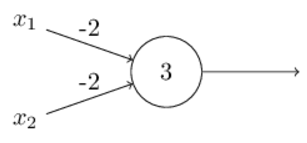
\includegraphics[scale=0.6]{Bilder/perceptron_example}
	\caption{Percetron mit zwei Eingaben -2 und einem Bias von 3.} 
	\label{fig:perceptron_example} 
\end{figure}

\noindent
Um das Verhalten des Perceptrons weiter zu untersuchen werden zum einen die Eingaben $x_1, x_2$  mit dem Wert 0 und zum anderen mit dem Wert -1 belegt. \\[0.2cm]
\hspace*{1.3cm}
$
\begin{array}[t]{lclll}
	(-2)*0+(-2)*0+3 & = & 3 & \geq & 0  \quad\rightarrow\quad \mathtt{output} := 1 \\[0.2cm]
	(-2)*1+(-2)*1+3 & = & -1  & < & 0 \quad\rightarrow\quad \mathtt{output} := 0
\end{array}
$
\\[0.2cm]
Das vorliegende Perceptron ist in der Lage das Verhalten eines $\mathtt{NAND}$ Gatters nachzubilden. Somit kann auf dessen Basis auch ein Halbaddierer, der die Addition von zwei Bits $x_1$ und $x_2$ durchführt, implementiert werden. Für die Berechnung wird die bitweise Summe $x_1 \oplus x_2$ gebildet, wobei ein $\mathtt{carry bit}$ den Wert 1 annimmt, sobald $x_1$ und $x_2$ den Wert 1 aufweisen.
\begin{figure}[hbt]
	\centering
	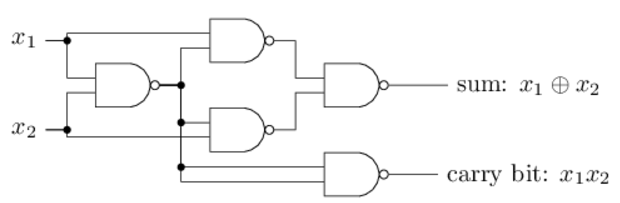
\includegraphics[scale=0.6]{Bilder/nand_gatter}
	\caption{Halbaddierer mit den Eingaben $x_1$ und $x_2$.} 
	\label{fig:nand_gatter} 
\end{figure}

\noindent
Um ein gleichwertiges Netzwerk abzuleiten, werden die $\mathtt{NAND}$ Gatter durch Perceptrons mit jeweils 2 Eingaben ersetzt. Hierbei weisen die Gewichtungen $w_1, w_2$ den Wert -2 und die Vorbelastung $b$ den Wert 3 auf. 
\begin{figure}[hbt]
	\centering
	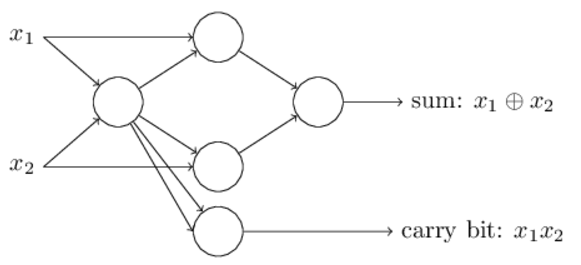
\includegraphics[scale=0.6]{Bilder/nand_gatter_perceptron}
	\caption{Halbaddierer-Aufbau mit Perceptrons.} 
	\label{fig:nand_gatter_perceptron} 
\end{figure}

\noindent
In einem weiteren Schritt wird die Abbildung eines $\mathtt{NAND}$ Gatter mit Perceptrons vereinfacht. Dazu werden mehrere Eingänge eines Perceptrons zu einem zusammengefasst, weshalb aus den zwei Eingaben -2 der Wert -4 resultiert. Ebenfalls werden die Eingaben in der Eingabeschicht des neuronalen Netzwerkes zusammengefasst, wobei jedoch durch diese Notation eine Eingabe nicht mit einem Perceptron gleichzustellen ist. Das vorliegende Netzwerk mit Perceptrons entspricht somit dem Aufbau eines Halbaddierers (siehe Abb. \ref{fig:nand_gatter_perceptron_simplified}). \\
\begin{figure}[hbt]
	\centering
	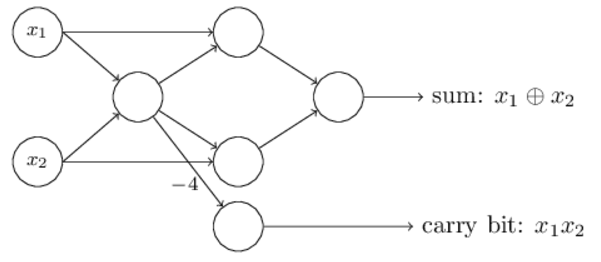
\includegraphics[scale=0.6]{Bilder/nand_gatter_perceptron_simplified}
	\caption{Vereinfachter $\mathtt{NAND}$ Gatter Aufbau mit Perceptrons.} 
	\label{fig:nand_gatter_perceptron_simplified} 
\end{figure}

\noindent
Wie im obigen Beispiel aufgezeigt, lassen sich mittels Perceptrons unterschiedliche Berechnungen durchführen. Auf diese Weise können implementierte Lernalgorithmen Gewichtungen sowie die Vorbelastung automatisch durch entsprechende Stimuli im Netzwerk anpassen und ermöglichen die Nutzung von künstlichen Neuronen.

\section{Sigmoid Neurons}
Für die Entwicklung lernender Algorithmen in einem Netzwerk, fällt die Betrachtung in dieser Arbeit auf die Erkennung von handgeschrieben Zahlen. Die Eingabe für das Netzwerk könnten die Raw Pixeldaten der eingescannten Bilder darstellen, welche die handgeschrieben Zahlen abbilden. Das Ziel an dieser Stelle ist, dass das Netzwerk anhand der Veränderungen von \textit{Gewichtungen} und der \textit{Vorbelastung} lernt eine korrekte Klassifizierung der Zahlen vorzunehmen. \\
Das Modifizieren der \textit{Gewichtungen} und der \textit{Vorbelastung} von Neuronen kann das Verhalten des Netzwerkes und deren Entscheidungsfindung zu Problemen beeinflussen. Angenommen die Erkennung und Klassifizierung einer Zahl wurde durch das Netzwerk falsch vorgenommen, so können durch kleine Veränderungen an den \textit{Gewichtungen} und der \textit{Vorbelastung} eine Korrektur durchgeführt werden. Dieses stetige Modifizieren der Werte über einen definierten Zeitraum ermöglicht ein lernendes Netzwerk (siehe Abb. \ref{fig:sigmoid_learning}). 
\begin{figure}[hbt]
	\centering
	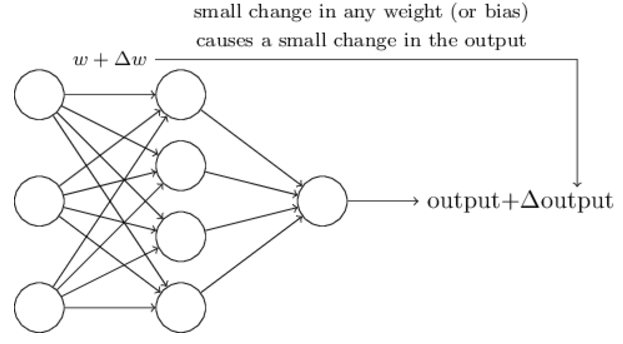
\includegraphics[scale=0.7]{Bilder/sigmoid_learning}
	\caption{Modifizieren von Weights und Biases schaffen lernendes Netzwerk.} 
	\label{fig:sigmoid_learning} 
\end{figure}

\noindent
Mit Hilfe der Einführung des Sigmoid Neurons soll der Fehler zur Klassifizierung von Zahlenwerten minimiert werden. Eine Änderung der Gewichtungen und der Vorbelastung bei diesem künstlichen Neuron soll nur marginale Änderungen an dem Ausgabewert $\mathtt{output}$ vornehmen. Diese Erweiterung des Neurons begünstigt ein Netzwerk selbständig die Klassifizierung von Zahlen zu optimieren. \\[0.2cm]
\hspace*{1.3cm}
$
\begin{array}[t]{lclll}
	\mathbf{w} + \Delta\mathbf{w} \quad\rightarrow\quad \mathtt{output} + \Delta\mathtt{output}
\end{array}
$
\\[0.2cm]

\noindent
Der Aufbau des Sigmoid Neurons ähnelt dem Perceptron, wobei das Neuron eine Anzahl von Eingabewerten $x_n$ mit $n \in \{1, \cdots ,m\}$ entgegennimmt und ausgehend von diesen Informationen den $\mathtt{output}$ ermittelt. Der wesentliche Unterschied zwischen diesen zwei Typen von Neuronen liegt in der differenzierbaren Funktion des Sigmoid Neurons zur Bestimmung des Ausgabewertes. Bei dem Sigmoid Neuron kann dieser alle Werte im Intervall $[0,1]$ annehmen. Weiterhin weist auch diese Art von Neuronen für jeden Eingabewert eine Gewichtung $w_n$ mit $n \in \{1, \cdots ,m\}$ sowie eine Vorbelastung auf. \\
Für die Berechnung des $\mathtt{output}$ wird in diesem Kontext die \textit{Sigmoid Funktion} $\sigma(z)$ angewendet.
\begin{equation}
	\sigma(z) \equiv \frac{1}{1+e^{-z}} \quad\mbox{mit}\quad z = \mathbf{w} \cdot \mathbf{x} + b
\end{equation}
Unter Berücksichtigung des Gewichtungsvektors \\[0.2cm]
\hspace*{1.3cm}
$
\begin{array}[t]{lclll}
	\mathbf{w} = \langle w_1, \cdots, w_m \rangle^\top
\end{array}
$
\\[0.2cm]
und des Eingabevektors \\[0.2cm]
\hspace*{1.3cm}
$
\begin{array}[t]{lclll}
	\mathbf{x} = \langle x_1, \cdots, x_m \rangle^\top
\end{array}
$
\\[0.2cm]
ergibt sich mit der Indexnotation 
\begin{equation}
	\sigma(z) \equiv \frac{1}{1+\exp(-\sum_j w_j x_j - b)}.
\end{equation}
Dabei weist das Sigmoid Neuron das gleiche Verhalten wie ein Perceptron auf, wenn eine Grenzwertbetrachtung durchführt wird. \\[0.2cm]
\hspace*{1.3cm}
$
\begin{array}[t]{lcll}
	\lim\limits_{z \to \infty}{\sigma(z)} & \approx & 1 \quad\quad bzw. \\[0.2cm]
	\lim\limits_{z \to -\infty}{ \sigma(z)} & \approx & 0
\end{array}
$
\\[0.2cm]
Dieses Verhalten wird weiterhin verdeutlicht, wenn die Betrachtung auf den folgenden Funktionsgraph fällt (siehe Abb. \ref{fig:sigmoid_plot}). Für große $z$ nimmt die Funktion den Wert 1 an und für kleine $z$ nimmt die Funktion den Wert 0 an.
\begin{figure}[hbt]
	\centering
	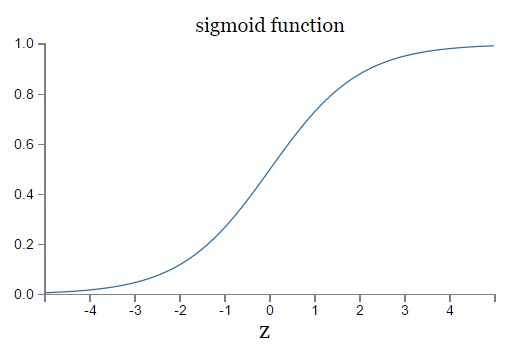
\includegraphics[scale=0.6]{Bilder/sigmoid_plot}
	\caption{Sigmoid Funktion $\sigma(z)$.} 
	\label{fig:sigmoid_plot} 
\end{figure}

\noindent
Die Vorteile der Sigmoid Funktion liegen in den marginalen Änderungen $\Delta w_j$ bei den Gewichtungen und $\Delta b$ bei der Vorbelastung, welche eine marginale Änderung am $\Delta\mathtt{output}$ vornehmen. Damit stellt $\Delta\mathtt{output}$ die lineare Funktion bezüglich der Änderungen  $\Delta w_j$ und $\Delta b$ in den Gewichtungen und der Vorbelastung dar.
\begin{equation}
	\Delta\mathtt{output} \equiv \sum_{j}{\frac{\partial\mathtt{output}}{\partial w_j}\Delta w_j+\frac{\partial\mathtt{output}}{\partial b}\Delta b}
\end{equation}
Diese Linearität begünstigt die Wahl von kleinen Änderungen in den Gewichtungen und der Vorbelastung, um das Verhalten für ein lernendes Netzwerk abzuleiten. \\

\noindent
Ein \textit{Feedforward Neural Network} besteht aus $L$ Schichten, wobei die Topologie des Netzwerkes durch $L \in \mathbb{N}$ und einer Liste $[m(1),\cdots ,m(L)]$ geben ist. $L$ bezeichnet die Anzahl der Schichten, während $m(l)$ mit $l \in \{2,\cdots ,L\}$ die Anzahl der Neuronen in der $l$-ten Schicht angibt. Somit ist erste Schicht des Netzwerks, die Eingabeschicht, über die Eingabedimension $m(1)$ und die Ausgabedimension über $m(L)$ definiert. \\
Jedes Neuron der $l$-ten Schicht hat über die Gewichtung eine Verbindung zu einem Neuron in der $(l+1)$-ten Schicht. Die Gewichtung $w_{j,k}^{(l)}$ stellt die Verbindung des $k$-ten Neurons in der $l-1$ Schicht zu dem $j$-ten Neuron in der $l$-ten Schicht. Die Gewichtungen in Schicht $L$ werden über die Gewichtungsmatrix $W^{(l)}$ der Schicht $l$ zusammengefasst. Die Matrix ist wie folgt definiert \\[0.2cm]
\hspace*{1.3cm}
$
\begin{array}[t]{lclll}
	W^{(l)} := \left( w_{j,k}^{(l)}\right)
\end{array}
$
\\[0.2cm]
und ist eine $m(l)\times m(l-1)$ Matrix, wobei \\[0.2cm]
\hspace*{1.3cm}
$
\begin{array}[t]{lclll}
	W^{(l)} \in \mathbb{R}^{m(l)\times m(l-1)}.
\end{array}
$
\\[0.2cm]
Weiterhin hat das $j$-te Neuron in Schicht $l$ eine Vorbelastung $b_j^{(l)}$. Die Vorbelastungen der Neuronen in Schicht $l$ werden über den Vorbelastungsvektor \\[0.2cm]
\hspace*{1.3cm}
$
\begin{array}[t]{lclll}
	\mathbf{b}^{(l)} := \langle b_1^{(l)},\cdots ,b_{m(l)}^{(l)}\rangle
\end{array}
$
\\[0.2cm]
zusammengefasst. Hieraus ergibt sich für das $j$-te Neuron der $l$-ten Schicht die Sigmoid Funktion $\sigma_j^{(l)}$, die wie folgt rekursiv definiert wird:
\begin{enumerate}
	\item Für die Eingabeschicht ergibt sich 
			\begin{equation}
        	\label{eq:feedforward1}
      			 \sigma_j^{(1)}(z) := x_j.
     		\end{equation}
    \item Für alle anderen Schichten ergibt sich
    		\begin{equation}
         	\label{eq:feedforward2}
         		\sigma_j^{(l)}(z) := 
             	\sum\limits_{k=1}^{m(l-1)} \left(w_{j,k}^{(l)}\cdot \sigma^{(l-1)}(z) + b_{j}^{(l)}\right) \quad \mbox{for all $l \in \{2, \cdots, L\}$}.
			\end{equation}
\end{enumerate}
Die Ausgabe des neuronalen Netzwerks für eine gegebene Eingabe $\mathbf{x}$ ist durch die Neuronen der Ausgabeschicht festgelegt. Diese werden über den Ausgabevektor $\mathbf{o} \in \mathbb{R}^{m(L)}$ mit \\[0.2cm]
\hspace*{1.3cm}
$
\begin{array}[t]{lclll}
	\mathbf{o}(x) := \langle \sigma_1^{(L)}(x),\cdots ,\sigma^{(L)}(z)\rangle = \sigma^{(L)}(x)
\end{array}
$
\\[0.2cm]
definiert. Unter Berücksichtigung der Gleichungen \ref{eq:feedforward1} und \ref{eq:feedforward2} kann nun nachvollzogen werden, wie Informationen das Netzwerk durchlaufen.
\begin{enumerate}
	\item  Der gegebene Eingabevektor $\mathbf{x}$ wird in der ersten und sogenannten Eingabeschicht des neuronalen Netzwerks gespeichert: \\[0.2cm]
\hspace*{1.3cm}
$
\begin{array}[t]{lclll}
	\sigma^{(1)}(z) := \mathbf{x}.
\end{array}
$
	\item Auf der zweiten Schicht liegt die erste Neuronenebene vor bei denen die Sigmoid Funktion zum Einsatz kommt: \\[0.2cm]
\hspace*{1.3cm}
$
\begin{array}[t]{lclll}
	\sigma^{(2)}(z) := W^{(2)}\cdot \sigma^{(1)}(z)+\mathbf{b}^{(2)} = W^{(2)}\cdot \mathbf{x}+\mathbf{b}^{(2)}.
\end{array}
$
\item Auf der dritten Schicht liegt die zweite Neuronenebene vor bei denen die Sigmoid Funktion zum Einsatz kommt: \\[0.2cm]
\hspace*{1.3cm}
$
\begin{array}[t]{lclll}
	\sigma^{(3)}(z) := W^{(3)}\cdot \sigma^{(2)}(z)+\mathbf{b}^{(3)} = W^{(3)}\cdot \left(W^{(2)}\cdot \mathbf{x}+\mathbf{b}^{(2)}\right)+\mathbf{b}^{(3)}.
\end{array}
$
\item Dieser Vorgang wird solange durchlaufen bis die Ausgabeschicht erreicht wird und die Ausgabe \\[0.2cm]
\hspace*{1.3cm}
$
\begin{array}[t]{lclll}
	\mathbf{o}(\mathbf{x}) := \sigma^{(L)}(z)
\end{array}
$
\end{enumerate}

\section{Stochastic Gradient Descent}
Für eine zuverlässige Klassifizierung der Zahlen wird ein Algorithmus benötigt, der die Bestimmung von Gewichtungen und der Vorbelastungen ...

\section{Backpropagation}

%\section{Netzwerk zur Klassifizierung von handgeschrieben Zahlen}

\chapter{Implementierung}

\section{Laden und Aufbereitung der MNIST Daten}
Für das Neuronale Netzwerk zur Erkennung von hangeschriebenen Zeichen zwischen werden Test- und Trainingsdaten der MNIST Datenbank genutzt. Die Datensätze können unter folgender Adresse gefunden werden: 
\\[0.2cm]
\hspace*{1.3cm}
\href{http://yann.lecun.com/exdb/mnist/}{http://yann.lecun.com/exdb/mnist/}
\\[0.2cm]
Da der MNIST Datensatz lediglich in Form von Binärdateien vorliegt und es in der aktuellen Version von SetlX nicht möglich ist Binärdateien zu lesen, wurde statt dem original Datensatz der umgewandelte Datensatz in Form einer CSV-Datei verwendet. Die Dateien können hier heruntergeladen werden:
\\[0.2cm]
\hspace*{1.3cm}
\href{https://pjreddie.com/projects/mnist-in-csv/}{https://pjreddie.com/projects/mnist-in-csv/}
\\[0.2cm]
Die Verwendung des CSV-Formats führt dazu, dass die Größe der Datensätze auf Grund fehlender Komprimierungen ansteigt. Ebenso wird das Einlesen der Datensätze langsamer, was an der eigentlichen Funktion des neuronalen Netzes allerdings nichts ändert und somit für dieses Projekt vertretbar ist. Eine Option das erste Problem zu umgehen wäre die Komprimierung in das Zip-Format und die Dekomprimierung zu Beginn des Startens des Programms. Da SetlX keine Unzip-Funktion für Dateien bietet, müsste hierbei allerdings Kenntnis über das jeweils vom Benutzer verwendete Betriebssystem gegeben sein und ebenso ob und wenn ja welches Programm hierfür zur Verfügung steht. Bei der Festlegung auf ein ein Kommandozeilen-Befehl (z.B. "gunzip" oder "unzip" für Linux-basierte PCs) würde somit die Betriebssystemunabhängigkeit verloren gehen.\\
Verwendet werden die CSV-Dateien $\mathtt{mnist\_test.csv}$ und $\mathtt{mnist\_train.csv}$. Die Traingsdaten umfassen insgesamt 60.000 Datensätze und die Testdaten 10.000 Datensätze. 
Die einzelnen Datensätze, also die handgeschriebenen Zeichen, sind in den Dateien in folgendem Format gespeichert:
\begin{center}
	$\mathtt{label, pixel1, pixel2, pixel3, ..., pixel784}$ \\
	$\mathtt{label, pixel1, pixel2, pixel3, ..., pixel784}$ \\
	...
\end{center}
Das heißt, in jeder Zeile befinden sich alle Daten zu einer Ziffer. Der erste Wert gibt den jeweiligen Wert an (z.B. 5) und darauf folgend befinden sich alle Pixel der Ziffer mit deren jeweiligen Graustufenwerten. Die Pixel werden der Reihe nach abgespeichert, wobei die "Leserichtung" einer Ziffer von links nach rechts und dann von oben nach unten ist.\\ \\
Um die Datensätze nun in SetlX importieren zu können, wird die Datei $\mathtt{csv\_loader.stlx}$ verwendet. Wird die Datei im SetlX-Interpreter ausgeführt, so liest sie die CSV-Dateien der Test- und Trainingsdaten (die Dateien müssen im selben Verzeichnis liegen und den oben erwähnten Namen haben) und speichert die Daten in den Variablen $\mathtt{test\_data}$ sowie $\mathtt{training\_data}$. Die Testdaten sind hierbei als Liste von Paaren in Form folgender Form abgelegt: \\
\hspace*{0.3cm}
$
\begin{array}[t]{lcll}
	[ \\[0.1cm]
	
	\hspace*{0.5cm}
	\begin{array}[t]{lcll}
    	[\mathtt{pixels},\ \mathtt{label}], \\[0.1cm]
    	[\mathtt{pixels},\ \mathtt{label}], \\[0.1cm]
    	... \\[0.1cm]
    \end{array}
    \\[0.1cm]
    
    ] \\[0.1cm]
\end{array}
$
\\[0.0cm]

\noindent
Hierbei ist $\mathtt{pixels}$ eine Liste mit Integer Werten zwischen 0 und 255. Der Wert des Zeichens wird in $\mathtt{label}$ als Integer gespeichert. \\ 
Die Trainingsdaten sind prinzipiell nach dem gleichen Prinzip aufgebaut, allerdings wird hier für spätere Auswertungszwecke der Wert der Ziffer nicht als konkrete Zahl gespeichert, sondern in vektorisierter Form. Der vektorisierte Wert einer Zahl wird hier durch einen Vektor dargestellt, dessen Inhalt immer 0 ist, außer an der $\mathtt{label+1}$-ten Stelle. Dies entspricht dann genau der Form der Ausgabe des Netzwerkes. Beispielhaft würde eine Ziffer mit dem Wert $7$ als folgender Vektor dargestellt werden: \\
$<<0\ 0\ 0\ 0\ 0\ 0\ 0\ 1\ 0\ 0>>$ \\

\noindent
Auf eine genaue Beschreibung der Implementierung des Ladevorgangs wird in dieser Studienarbeit verzichtet, da hierbei keine komplexen Funktionen angewandt wurden und das Verfahren nicht relevant für das Verständnis neuronaler Netze an sich ist.

\section{Implementierung des neuronalen Netzes}
Dieser Abschnitt beschreibt die eigentliche Implementierung des neuronalen Netzwerkes zur Erkennung von handgeschriebenen Ziffern in SetlX. Um den Code möglichst kompakt zu halten, wurden die in den Originaldateien enthaltenen Kommentarzeilen in dieser Seminararbeit zum größten Teil entfernt.
Bei der Umsetzung des Netzwerkes in SetlX wird der SGD-Algorithmus als Lernmethode des Netzwerkes benutzt. Die im vorherigen Kapitel importierten Daten des MNIST-Datensatzes dienen als Grundlage der Ziffernerkennung. 
Das Netzwerk wird als Klasse in SetlX angelegt und enthält die folgenden Membervariablen:

\begin{enumerate}
\item $\mathtt{mNumLayers}$: Anzahl der Schichten des aufzubauenden Netzwerkes 
\item $\mathtt{mSizes}$: Aufbau des Netzwerkes in Listenform. Bsp.: $[784, 30, 10]$ beschreibt ein Netzwerk mit 784 Eingabe-Feldern, 30 Neuronen in der zweiten Schicht und 10 Ausgabe-Neuronen
\item $\mathtt{mBiases}$: Alle Vorbelastungen des Netzwerkes (genauer Aufbau wird im Folgenden erläutert)
\item $\mathtt{mWeights}$: Alle Gewichte des Netzwerkes (genauer Aufbau wird im Folgenden erläutert)
\end{enumerate}

\noindent
Die Initialisierung des Netzwerkes zur Ziffernerkennung erfolgt durch folgende Befehle:
\begin{Verbatim}[ frame         = lines, 
                  framesep      = 0.3cm, 
                  firstnumber   = 1,
                  labelposition = bottomline,
                  numbers       = left,
                  numbersep     = -0.2cm,
                  xleftmargin   = 0.8cm,
                  xrightmargin  = 0.8cm,
                ]
    net := network([784, 30, 10]);
    net.init();
\end{Verbatim}
Als Übergabeparameter bei der Erstellung eines Netzwerk-Objektes wird die Struktur des Netzwerkes in Form einer Liste übergeben. Diese wird dann lediglich $\mathtt{mSizes}$ zugeordnet und basierend hierrauf wird $\mathtt{mNumLayers}$ ermittelt.
Die $\mathtt{init()}$-Funktion der $\mathtt{network}$-Klasse wird verwendet um die Gewichte und Vorbelastungen des Netzwerkes initial zufällig zu belegen. Hiermit werden Ausgangswerte gesetzt, welche später durch das Lernen des Netzwerkes angepasst werden.
Im Folgenden sind die verwendeten Funktionen, welche während der Gewichts- und Vorbelastungs-Initialisierung verwendet werden, zu sehen.
\begin{Verbatim}[ frame         = lines, 
                  framesep      = 0.3cm, 
                  firstnumber   = 1,
                  labelposition = bottomline,
                  numbers       = left,
                  numbersep     = -0.2cm,
                  xleftmargin   = 0.8cm,
                  xrightmargin  = 0.8cm,
                ]
    init := procedure() {
        computeRndBiases();
        computeRndWeights();
    };
    computeRndBiases := procedure() {
        this.mBiases := [ 
            computeRndMatrix(1, mSizes[i]) : i in [2..mNumLayers] 
        ];
    };
    computeRndWeights := procedure() {
        this.mWeights := [ 
            computeRndMatrix(mSizes[i], mSizes[i+1]) : i in [1..mNumLayers-1] 
        ];
    };
    computeRndMatrix := procedure(row, col) {
        return la_matrix([
            [ ((random()-0.5)*2)/28 : p in [1..row] ] : q in [1..col]
        ]);
    };
\end{Verbatim}

\begin{enumerate}
\item $\mathtt{init()}$: In der Funktion werden die Vorbelastungen und Gewichtungen des Netzwerkes zu Beginn initialisiert
\item $\mathtt{computeRndBiases()}$: Die Funktion befüllt die Variable mBiases mit zufälligen Werten. Der für das Netzwerk benötigte Aufbau der Vorbelastungen entspricht folgender Form: \\
$[ \\ 
<<\ <<\mathtt{Bias\_Schicht2\_Neuron1}>>\ <<\mathtt{Bias\_Schicht2\_Neuron2}>>\ ...\ >>, \\
<<\ <<\mathtt{Bias\_Schicht3\_Neuron1}>>\ ...\ >>, \\
 ...\ ]$ \\
Das heißt es kann auf die Vorbelastungen mit folgendem Schema in SetlX zugegriffen werden: \\
\begin{center}
	$\mathtt{mBiases[Schicht][Neuron][1]}$
\end{center}
Hierbei ist zu beachten, dass der letzte Index immer 1 ist, da jedes Neuron nur eine einzige Vorbelastung besitzt und die Vorbelastungen als Matrix abgelegt werden. Die Verwendung des Matrix-Datentyps wurde bewusst, auf Grund späterer Berechnungen mit Hilfe der $\mathtt{la\_hadamard()}$-Funktion, gewählt. Da es sich bei der Eingabe-Schicht des Netzwerkes nicht um Sigmoid-Neuronen handelt, sondern lediglich um Eingabewerte, werden hierfür keine Vorbelastungen benötigt. Deshalb wird bei der Erstellung der zufälligen Vorbelastungen nur $[2..\mathtt{mNumLayers}]$ (also alle Schichten außer der Ersten) betrachtet.
\item $\mathtt{computeRndWeights()}$: Diese Funktion ist equivalent zu der Vorbelastungs-Funktion, lediglich wird die Struktur der Gewichte mit folgenden Zugriffmsmöglichkeiten angelegt: \\
\begin{center}
	$\mathtt{mWeights[Schicht][Neuron][Gewicht]}$
\end{center}
\item $\mathtt{computeRndMatrix()}$: Diese Hilfsfunktion dient zur Erstellung der Struktur der Gewichte und Vorbelastungen in den zuvor vorgestellten Funktionen. Auf Grund der Verwendung der $\mathtt{la\_hadamard()}$-Funktion, welche im weiteren Programm benötigt wird, wurde sich für die Verwendung des Matrix-Datentyps statt eines Vektors entschieden. Die Funktion enthält als Parameter eine Matrix-Struktur mittels der Anzahl von Reihen und Spalten. Zurückgegeben wird die zugehörige Matrix mit zufälligen Werten zwischen $-1/28$ und $1/28$. Der Wert 28 ergibt sich aus der Größe des Eingabevektors (28x28 Pixel).  Die übergebende Struktur hat die Form $\mathtt{[x,y]}$, wobei $\mathtt{x}$ die Anzahl der Spalten und $\mathtt{y}$ die Anzahl der Zeilen angibt. \\
Bsp.: $s := [1,2]\ \rightarrow\ <<\ <<x>>\ <<y>>\ >>$ und $s := [2,1]\ \rightarrow\ <<\ <<x\ y>>\ >>$
\end{enumerate}

\noindent
Sei nun $W$ die Matrix der Gewichte und $B$ die Matrix aller Vorbelastungen und $\mathbf{a}$ bezeichnet den Aktivierungsvektor der vorherigen Schicht, also deren Ausgabe (zu Beginn also die Pixel der Eingabe). Nach Gleichung \textcolor{red}{[ToDo: Verlinkung zu Theorieteil]} zur Berechnung einer Sigmoid-Ausgabe lässt sich nun folgende Formel aufstellen: 
\begin{equation}\label{eq:feedforward_impl}
	\mathbf{a}^{(l)} = \sigma(W^{(l)}\cdot \mathbf{a}^{(l-1)} + B^{(l)})
\end{equation}
\noindent
Hierbei bezeichnet $\mathbf{a}^{(l)}$ den Ausgabe-Vektor der aktuellen Schicht, welcher dann der nächsten Schicht weitergeleitet wird (feedforwarding). Nachfolgend sind die Implementierungen der Sigmoid-Funktionen sowie dem Feedforwarding zu sehen.
\begin{Verbatim}[ frame         = lines, 
                  framesep      = 0.3cm, 
                  firstnumber   = 1,
                  labelposition = bottomline,
                  numbers       = left,
                  numbersep     = -0.2cm,
                  xleftmargin   = 0.8cm,
                  xrightmargin  = 0.8cm,
                ]
    feedforward := procedure(a) {
        for( i in {1..#mBiases} ) { 
            a := sigmoid( mWeights[i]*a + mBiases[i] );
        }
        return a;
    };                            
    sigmoid := procedure(z) {
        return la_vector([ 1.0/(1.0 + exp(- z[i] )) : i in [1..#z] ]);
    };
    sigmoid_prime := procedure(z) {
        s := sigmoid(z); 
        return la_matrix([ [ s[i] * (1 - s[i]) ] : i in [1..#s] ]);
    };
\end{Verbatim}
\begin{enumerate}
\item $\mathtt{feedforward(a)}$: Anwendung der Gleichung \eqref{eq:feedforward_impl} auf alle Schichten des Netzwerkes angewandt. Zurückgegeben wird die resultierende Ausgabe jedes Neurons der letzten Schicht in vektorisierter Form.
\item $\mathtt{sigmoid(z)}$: Diese Funktionen nimmt einen Vektor $\mathtt{z}$ und berechnet mit Hilfe der Sigmoid-Formel (siehe Formel \textcolor{red}{[ToDo: Verlinkung zu Theorieteil]}) die Ausgabe der Neuronen in vektorisierter Form.
\item $\mathtt{sigmoid\_prime(z)}$: Für einen gegebenen Vektor $\mathtt{z}$ wird die Ableitung der Sigmoid-Funktion (nach Formel \textcolor{red}{[ToDo: Verlinkung zu Theorieteil]}) berechnet und in Form einer Matrix (Matrix-Form auf Grund späterer Berechnung mit $\mathtt{la\_hadamard()}$) zurückgegeben.
\end{enumerate}
\noindent
Die Feedforward-Funktion dient also dazu, die Eingabewerte durch das gesamte Netzwerk durchzureichen und die daraus resultierende Ausgabe zu ermitteln. Als nächstes wird der Algorithmus diskutiert, durch welchem es dem Netzwerk ermöglicht wird zu \glqq lernen\grqq. Hierfür wird der SGD-Algorithmus verwendet. Die Implementierung des SGDs in SetlX ist nachfolgend aufgezeigt und wird nun im Detail erläutert.

\begin{Verbatim}[ frame         = lines, 
                  framesep      = 0.3cm, 
                  firstnumber   = 1,
                  labelposition = bottomline,
                  numbers       = left,
                  numbersep     = -0.2cm,
                  xleftmargin   = 0.8cm,
                  xrightmargin  = 0.8cm,
                ]
    sgd := procedure(training_data, epochs, mini_batch_size, eta, test_data) {
        if(test_data != null) {
            n_test := #test_data; 		
        }
        n := #training_data;		
        for(j in {1..epochs}) {
            training_data := shuffle(training_data);
            mini_batches := [ 
                training_data[k..k+mini_batch_size-1] : k in [1,mini_batch_size..n] 
            ];		
            for(mini_batch in mini_batches) {
                update_mini_batch(mini_batch, eta);
            } 		
            if(test_data != null) {
                ev := evaluate(test_data);
                print("Epoch $j$: $ev$ / $n_test$");
            }
            else {
                print("Epoch $j$ complete");
            }
        }
    };
\end{Verbatim}
\begin{enumerate}
\item Zeile 1: Übergabeparameter der Funktion sind die Trainingsdatensätze (Liste von Tupeln $\mathtt{[x,y]}$ mit $\mathtt{x}$ als Eingabewerten und $\mathtt{y}$ als gewünschtem Ergebnis), die Anzahl der Epochen (Integer-Wert), die Größe der Mini-Batches (Integer-Wert), die gewünschte Lernrate (Fließkomma-Wert) und den optionalen Testdatensätzen (äquivalenter Aufbau zu Trainingsdaten).
\item Zeile 6: Der nachfolgende Programmcode wird entsprechend der übergebenen Epochenanzahl mehrfach ausgeführt.
\item Zeile 7-10: Zuerst werden alle Trainingsdaten zufällig vermischt und anschließend Mini-Batches (also Ausschnitte aus dem Gesamtdatensatz) der vorher festgelegten Größe aus den Trainingsdaten extrahiert. Somit wird eine zufällige Belegung von Mini-Batches garantiert. Alle Mini-Batches werden in Listenform in der Variablen $\mathtt{mini\_batches}$ gespeichert.
\item Zeile 11-13: Anschließend wird für jeden Mini-Batch aus $\mathtt{mini\_batches}$ eine Iteration des Gradient Descent Algorithmus angewendet. Dies geschieht mit Hilfe der Funktion $\mathtt{update\_mini\_batches}$, welche im nächsten Schritt ausführlicher erläutert wird. Zweck der Funktion ist es die Gewichte und Vorbelastungen des Netzwerkes mit Hilfe einer Iteration des SGD-Algorithmus anzupassen. Die Basis für diese Anpassung liefert der übergebene Mini-Batch und die Lernrate.
\item Zeile 14-20: Dieser Programmcode dient zur Ausgabe auf der Konsole und teilt dem Benutzer die aktuelle Anzahl an korrekt ermittelten Datensätzen der Trainingsdaten nach jeder Epoche mit. Hierfür wird die Hilfsfunktion $\mathtt{evaluate}$ verwendet, welche unter Berücksichtigung des aktuellen Netzwerkzustandes die Outputs ermittelt, welcher bei Eingabe der Testdaten durch das Netzwerk errechnet wurden (genaue Implementierung folgt). Sollten der $\mathtt{sgd}$-Funktion keine Testdaten übergeben worden sein, so entfällt diese Ausgabe.
\end{enumerate}

\noindent
Die in der SGD-Funktion erwähnte Hilfsfunktion $\mathtt{update\_mini\_batches}$ dient dazu, auf einem gegebenen Testdatensatz (Mini-Batch) eine Iteration des Gradient Descent Algorithmus anzuwenden. Zur Berechnung des Gradienten wird Backpropagation genutzt.
\begin{Verbatim}[ frame         = lines, 
                  framesep      = 0.3cm, 
                  firstnumber   = 1,
                  labelposition = bottomline,
                  numbers       = left,
                  numbersep     = -0.2cm,
                  xleftmargin   = 0.8cm,
                  xrightmargin  = 0.8cm,
                ]
    update_mini_batch := procedure(mini_batch, eta) {
        nabla_b := [ 0*mBiases[i] : i in {1..#mBiases}];
        nabla_w := [ 0*mWeights[i] : i in {1..#mWeights}];
        for([x,y] in mini_batch) {
            [delta_nabla_b, delta_nabla_w] := backprop(x,y);
            nabla_b := [ nabla_b[i] + delta_nabla_b[i] : i in {1..#nabla_b} ];
            nabla_w := [ nabla_w[i] + delta_nabla_w[i] : i in {1..#nabla_w} ];
        }
        this.mWeights := [ 
            mWeights[i] - eta/#mini_batch * nabla_w[i] : i in {1..#mWeights} 
        ];
        this.mBiases := [ 
            mBiases[i] - eta/#mini_batch * nabla_b[i] : i in {1..#mBiases} 
        ];
    };
\end{Verbatim}
\begin{enumerate}
\item Zeile 1: Der Funktion wird ein Mini-Batch aus der SDG-Funktion in Listenform mitgegeben. Die jeweiligen Datensätze der Liste bestehen bestehen aus Tupeln der Form $[x,y]$, wobei $x$ die Pixel des jeweiligen Zeichens darstellt und $y$ der erwartete Wert des Zeichens ist.
\item Zeile 2-3: Hier werden die Variablen $\mathtt{nabla\_b}$ und $\mathtt{nabla\_w}$ als Listen mit 0-en initialisiert. Die Länge der Listen entspricht jeweils der Zeilenanzahl der Gewichts- und Vorbelastungs-Matrizen. $\mathtt{nabla\_b}$ und $\mathtt{nabla\_w}$ stehen für die Gradienten der Gewichte und Vorbelastungen des Netzwerkes.
\item Zeile 5: Auf jedes Tupel $[x,y]$ der mitgegebenen Testdaten wird nun der Backpropagation-Algorithmus angewendet. Dieser dient dazu den Gradienten der Kostenfunktion möglichst schnell und effizient zu berechnen. Die Implementierung von Backpropagation folgt im Anschluss.
\item Zeile 6-7: Die durch die Backpropagation ermittelten Gradienten für die Gewichte und Vorbelastungen werden in den entsprechenden Variablen gespeichert.
\item Zeile 9-14: Nachdem die Gradienten durch jeden Datensatz des Mini-Batches angepasst wurden, werden am Ende der Funktion nun die Gewichte und Vorbelastungen des Netzwerkes entsprechend des Ergebnisses angepasst. Hierfür werden folgende Formeln verwendet:
\begin{equation}
	W' = W - \frac{\eta}{m}\cdot \nabla W \\
	B' = B - \frac{\eta}{m}\cdot \nabla B
\end{equation}
Hierbei bezeichnet $W$ die Gewichtsmatrix und $B$ die Vorbelastungsmatrix des Netzwerkes. Die Lernrate wird durch $\eta$ dargestellt und $m$ bezeichnet die Größe der betrachteten Testdaten. Die Lernrate wird durch den Benutzer vorgegeben und der Funktion als Parameter übergeben. $m$ kann durch die Größe des Mini-Batches ermittelt werden. \textcolor{red}{[ToDo: Verweis auf vorherige Formeldefinition, wenn vorhanden]}
\end{enumerate}

\noindent
Im nächsten Abschnitt wird die Implementierung des Backpropagation Algorithmus vorgestellt. Dieser dient dazu den Gradienten der Gewichte und Vorbelastungen zu berechnen, damit das Netzwerk anhand der Testdatensätze lernen kann. Zur Erinnerung sind hier noch einmal die vier grundlegenden Formeln des Algorithmus erwähnt:
\begin{equation} \label{eq:BP1_impl}
	\boldsymbol{\varepsilon}^{(L)} = (\mathbf{a}^{(L)} - \mathbf{y}) \odot S'\bigl(\mathbf{z}^{(L)}\bigr)  
\end{equation}
\begin{equation} \label{eq:BP2_impl}
	\boldsymbol{\varepsilon}^{(l)} = \Bigl(\bigl(W^{(l+1)}\bigr)^\top \cdot \boldsymbol{\varepsilon}^{(l+1)}\Bigr) \odot
  S'\bigl(z^{(l)}\bigr) \quad \mbox{für alle $l \in \{2, \cdots, L-1\}$}.
\end{equation}
\begin{equation} \label{eq:BP3_impl}
	\nabla_{\mathbf{b}^{(l)}} C_{\mathbf{x}, \mathbf{y}} = \boldsymbol{\varepsilon}^{(l)}
  \quad \mbox{für alle $l \in \{2, \cdots,l\}$}
\end{equation}
\begin{equation} \label{eq:BP4_impl}
	\nabla_{W^{(l)}} C_{\mathbf{x}, \mathbf{y}} = \boldsymbol{\varepsilon}^{(l)} \cdot \bigl(\mathbf{a}^{(l-1)}\bigr)^\top
  \quad \mbox{für alle $l \in \{2, \cdots,l\}$}
\end{equation}
Nachfolgend ist die eigentlichen Umsetzung in SetlX mit einigen Erläuterungen zu sehen.
\begin{Verbatim}[ frame         = lines, 
                  framesep      = 0.3cm, 
                  firstnumber   = 1,
                  labelposition = bottomline,
                  numbers       = left,
                  numbersep     = -0.2cm,
                  xleftmargin   = 0.8cm,
                  xrightmargin  = 0.8cm,
                ]
    backprop := procedure(x,y) {
        nabla_b := [ 0 : i in {1..#mBiases}];
        nabla_w := [ 0 : i in {1..#mWeights}];
        activation := x;
        activations := [ la_matrix(x) ];
        len_act := #activations;
        activations += [0 : i in [1..#mBiases]];
        zs := [0 : i in [1..#mBiases]];		
        for(i in {1..#mBiases}) {
            zs[i] := mWeights[i] * activation + mBiases[i];	
            activation := sigmoid(z[i]);
            activations[i + len_act] := la_matrix(activation);
        }
        cdm := la_matrix( cost_derivative(activations[-1], y) );
        epsilon := la_hadamard( cdm, sigmoid_prime(zs[-1]));
        lb := #nabla_b;
        lw := #nabla_w;
        nabla_b[lb] := epsilon;	
        nabla_w[lw] := epsilon * activations[-2]!;				
        for( l in {2..mNumLayers-1} ) {
            sp := sigmoid_prime(zs[-l]);	
            epsilon := la_hadamard( mWeights[-l+1]! * epsilon, sp );
            nabla_b[lb-l+1] := epsilon;
            nabla_w[lw-l+1] := epsilon * activations[-l-1]!;
        }
        return [nabla_b, nabla_w];
    };
\end{Verbatim}
\begin{enumerate}
\item Zeile 1: Der Funktion werden Datensätze in Listenform mitgegeben. Die Datensätze bestehen aus Tupeln der Form $[x,y]$, wobei $x$ die Pixel des jeweiligen Zeichens darstellt und $y$ der tatsächliche Wert des Zeichens ist.
\item Zeile 2-3: Initialisierung der Gradienten-Variablen $\mathtt{nabla\_b}$ und $\mathtt{nabla\_w}$ mit 0-en.
\item Zeile 4-7: Die Variable $\mathtt{activiation}$ enthält den aktuellen Eingabevektor der vorherigen Schicht und wird für das Feedforwarding benötigt. Zu Beginn der Funktion entspricht $\mathtt{activiation}$ dem Pixel-Vektor der Eingabe, also $x$. $\mathtt{activiations}$ speichert die Aktivierungsvektoren aller Schichten. Der erste Wert der Liste wird mit dem Eingabevektor belegt. Aus Performance-Gründen wird die Variabel wieder mit 0-en initialisiert, um ein späteres Anhängen an die Liste zu vermeiden (einfügen, statt anhängen).
\item Zeile 8: $\mathtt{zs}$ bezeichnet die Lister aller z-Vektoren und wird mit 0-en initialisiert. Ein z-Vektor beinhaltet alle in der jeweiligen Schicht durch die entsprechenden Werte (Gewichte und Vorbelastungen) gewichteten Eingaben. Dies entspricht also der späteren Eingabewert der Sigmoid-Funktion. Zur Veranschaulichung der z-Vektoren und deren Bedeutung dient folgende Formel:
\begin{equation} \label{eq:zvector_impl}
	\mathbf{a}^{(l+1)} = \sigma(\mathbf{z})
\end{equation} 
Hierbei bezeichnet $\mathbf{a}^{(l+1)}$ den Aktivierungsvektor der nächsten Schicht.
\item Zeile 10-13: Für jede Schicht des Netzwerkes wird der entsprechende z-Vektor entsprechend der Gleichungen \eqref{eq:feedforward_impl} und \eqref{eq:zvector_impl} berechnet und der Liste $\mathtt{zs}$ hinzugefügt. Mit Hilfe des aktuellen z-Vektors kann der Aktivierungsvektor jeder Schicht berechnet werden. Alle Aktivierungsvektoren des Netzwerkes werden pro Schicht in $\mathtt{activiations}$ abgelegt. Um später mit den Aktivierungsvektoren besser rechnen zu können, werden die vektorisierten Aktivierungen in Matrixform in $\mathtt{activiations}$ abgelegt.
\item Zeile 15-16: Diese Zeilen stellen die Implementierung der ersten Gleichung des Backpropagation-Algorithmus \eqref{eq:BP1_impl} dar. Hierbei bezeichnet $\mathtt{epsilon}$ den Ausgabefehler $\boldsymbol{\varepsilon}^{(L)}$ des Netzwerkes. Um diesen berechnen zu können, wird die Hilfsfunktion $\mathtt{cost\_derivate}$ aufgerufen, welche den erwarteten Ausgabevektor $y$ von dem letzten Aktivierungsvektor (also die Ausgabe des Netzwerkes) subtrahiert. Da die Hadamard-Funktion von SetlX lediglich Matrizen als Parameter akzeptiert und $\mathtt{cost\_derivate}$ einen Vektor berechnet, muss dieser noch mittels $\mathtt{la\_matrix}$ in eine Matrix umgewandelt werden.
\item Zeile 17-18: Die Variablen $\mathtt{lb}$ und $\mathtt{lw}$ bezeichnen jeweils die Länge der Gewichts- und Vorbelastungslisten. Diese Variablen werden im Anschluss benötigt, da es in SetlX zwar möglich ist eine Liste oder eine Matrix von hinten mittels negativem Index (z.B. $a[-1]$) zu lesen, allerdings nicht zu beschreiben.
\item Zeile 19-20: Berechnung der Gradienten der Gewichte und Vorbelastung der Ausgabeschicht mittels der Formeln \eqref{eq:BP3_impl} und \eqref{eq:BP4_impl}.
\item Zeile 21-24: Dieser Code beschreibt die Berechnung der Gradienten für alle Schichten zwischen der zweiten und der Vorletzten in rückwärtiger Reihenfolge (also in unserem Netzwerkaufbau gilt für die Schleife: $l \in {2}$). Zunächst wird wieder der Ausgabefehler $\boldsymbol{\varepsilon}^{(L)}$ berechnet. Dies geschieht in Zeile 24 nach Formel \eqref{eq:BP2_impl}. Da wir in der Schleife mit negativen Indizes arbeiten, entspricht $\mathtt{epsilon}$ in jeder Iteration der nächsthöheren Schicht. Zeile 25 und 26 entsprechen den Formeln \eqref{eq:BP3_impl} und \eqref{eq:BP4_impl} und passen die Gradientenvariablen entsprechend an. Hierbei ist zu beachten, dass der Ausdruck "$\mathtt{lb-l+1}$" dem Ausdruck "$\mathtt{-l}$" entspricht. Da wie erwähnt ein Schreiben von Matrizen und Arrays mit negativen Indizes nicht möglich ist, musste auf die Werte mit einem positiven Index zugegriffen werden.
\item Zeile 28: Die Funktion liefert als Rückgabeparameter die entgültigen Gradienten der Netzwerkgewichte und -vorbelastungen, welche anschließend in der SGD-Funktion für den Gradientenabstieg verwendet werden.
\end{enumerate}

\noindent
Als Letztes wird die Funktion $\mathtt{evaluate}$ diskutiert, welche in der $\mathtt{sgd}$-Funktion aufgerufen wurde und dazu dient die Anzahl der vom Netzwerk korrekt ermittelten Datensätze zu berechnen. Die Funktion ist durch folgenden Code gegeben:
\begin{Verbatim}[ frame         = lines, 
                  framesep      = 0.3cm, 
                  firstnumber   = 1,
                  labelposition = bottomline,
                  numbers       = left,
                  numbersep     = -0.2cm,
                  xleftmargin   = 0.8cm,
                  xrightmargin  = 0.8cm,
                ]
    evaluate := procedure(test_data) {
        test_results := [[argmax(feedforward(x)) - 1, y]: [x, y] in test_data];	
        return #[1 : [x,y] in test_results | x == y];
    };
    argmax := procedure(x) {
        [maxValue, maxIndex] := [x[1], 1];
        for (i in [2 .. #x] | x[i] > maxValue) {
            [maxValue, maxIndex] := [x[i], i];
        }
        return maxIndex;
    };
\end{Verbatim}
\begin{enumerate}
\item Zeile 1: Der Funktion werden Datensätze in Listenform mitgegeben. Die Datensätze bestehen aus Tupeln der Form $[x,y]$, wobei $x$ die Pixel des jeweiligen Zeichens darstellt und $y$ der Wert des Zeichens ist.
\item Zeile 2: $\mathtt{test\_results}$ speichert die vom Netzwerk ermittelte Ausgabe, sowie die tatsächliche Ausgabe in Tupelform für jeden Datensatz. Mit Hilfe der bereits besprochenen Feedforward-Funktion wird zunächst die vektorisierte Ausgabe des Netzwerkes für den jeweiligen Datensatz berechnet. Anschließend wird mit Hilfe der $\mathtt{argmax()}$-Funktion der Index des maximalen Wertes im Vektor ermittelt. Die ermittelte Ziffer ergibt sich nun aus dem Index subtrahiert mit 1, da die Ziffern mit 0 beginnend im Ausgabevektor gespeichert sind. In die Variable $\mathtt{test\_results}$ wird letztendlich der errechnete Wert sowie der tatsächliche Wert ($y$) gespeichert.
\item Zeile 3: Die Funktion gibt im Anschluss die Anzahl aller übereinstimmenden Ergebnisse in $\mathtt{test\_results}$ zurück.
\item Zeile 5-11: Die Funktion $\mathtt{argmax()}$ ermittelt in einem Vektor oder einer Liste den Index des größten darin enthaltenen Wertes. Hierbei wird mit einer Schleife über die komplette Liste oder den kompletten Vektor iteriert und der aktuell höchste Wert mit entsprechendem Index in den Variablen $\mathtt{maxValue}$ und $\mathtt{maxIndex}$ gespeichert. Zurückgegeben wird der somit gefundene Index.
\end{enumerate}

\noindent
Eine vorgefertigte Prozedur zur Initialisierung des benötigten Netzwerkes mit Beispielparametern befindet sich in der Datei $\mathtt{start.stlx}$, welche mit dem Befehl 
\begin{center}
	$\mathtt{setlx\ start.stlx}$ 
\end{center}
über die Konsole gestartet werden kann.

\section{Animation}
In diesem Abschnitt der Arbeit wird auf die Implementierung der grafischen Ausgabe des neuronalen Netzwerks zur Erkennung von handgeschriebenen Zahlen in SetlX eingegangen. Das Ziel ist die grafische Aufbereitung der Daten aus dem Hauptprogramm. Es bildet hierbei die folgenden Informationen ab: 
\begin{itemize}
\item Aufbau des neuronalen Netzwerks.
\item Betrachtung des Untersuchungsbereich eines Neurons in der verborgenen Schicht.
\item Betrachtung des Untersuchungsbereich aller Neuronen der verborgenen Schicht.
\item Betrachtung des Untersuchungsbereich aller Neuronen für eine Eingabe $\mathbf{x}$ aus den Testdaten.
\end{itemize}
\vspace{0.5cm}
\noindent
Die folgenden Befehle ermöglichen die einzelnen Funktionalitäten in der Anwendung anzusteuern:
\begin{center}
\begin{tabular}{lp{8cm}}
\textbf{Eingabebefehl}   & \textbf{Erklärung} \\
\hline \\
$\mathbf{0}$      & Animation für den Aufbau des Netzwerks mit den unterschiedlichen Schichten z.B. $[784,30,19]$  \\[0.2cm]
$\mathbf{1-30}$   & Animation für den Untersuchungsbereich des angesteuerten Neurons $n$ im Hidden-Layer mit $n \in \{1..30\}$ des entsprechenden Netzwerk  \\[0.2cm]
$\mathbf{101-(\mathtt{mTestDataSize}+100})$  & Animation für den Untersuchungsbereich aller Neuronen für eine gegeben Zahl $x$ aus den Testdaten  \\[0.2cm]
$\mathbf{1000}$   & Animation für den Untersuchbereichs der einzelnen Neuronen  \\
\end{tabular}
\end{center}
\vspace{0.5cm}

\noindent 
Mit dem \textbf{Eingabebefehl 0} wird dynamisch der Aufbau des angewendeten neuronalen Netzwerks dem Anwender repräsentiert (siehe Abb. \ref{fig:animation_network_default}). Wie bereits im Theorieteil dieser Arbeit beschrieben, besteht das neuronale Netzwerk aus einer Eingabeschicht, einer oder mehrerer verborgener Schichten und einer Ausgabeschicht. \\
Die Eingabe für das Netzwerk ist eine handgeschriebene Zahl mit der Bildgröße von $28 \times 28$ Pixeln. Jedes Pixel stellt eine Eingabe des neuronalen Netzwerks dar, wobei 784 Eingaben aus der Bildgröße resultieren (siehe Abb. \ref{fig:MNIST-Matrix}). Diese werden für die Animation ebenfalls wie das Ursprungsbild in der Form eines Quadrats abgebildet. Weiterhin ist der Aufbau und die Verbindungen zwischen den Neuronen der verborgenen Schicht und der Ausgabeschicht dargestellt. \\

\begin{figure}[hbt]
	\centering
	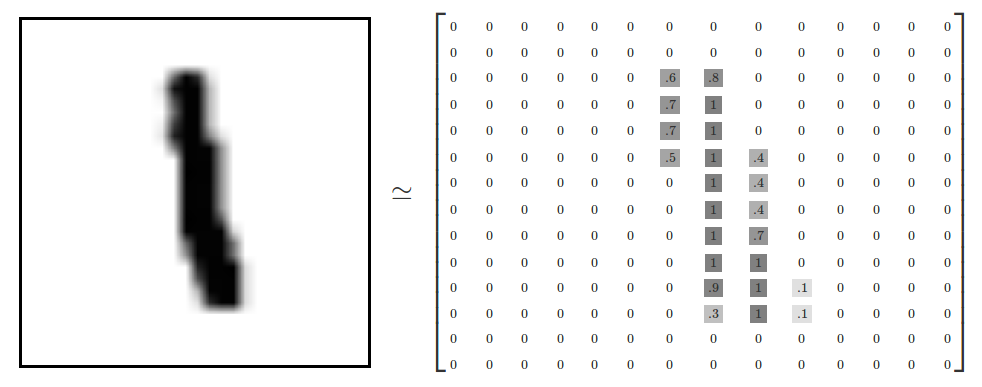
\includegraphics[scale=0.32]{Bilder/MNIST-Matrix}
	\caption{Eingabe in das neuronale Netzwerk.} 
	\label{fig:MNIST-Matrix} 
\end{figure}

\begin{figure}[!hbt]
	\centering
	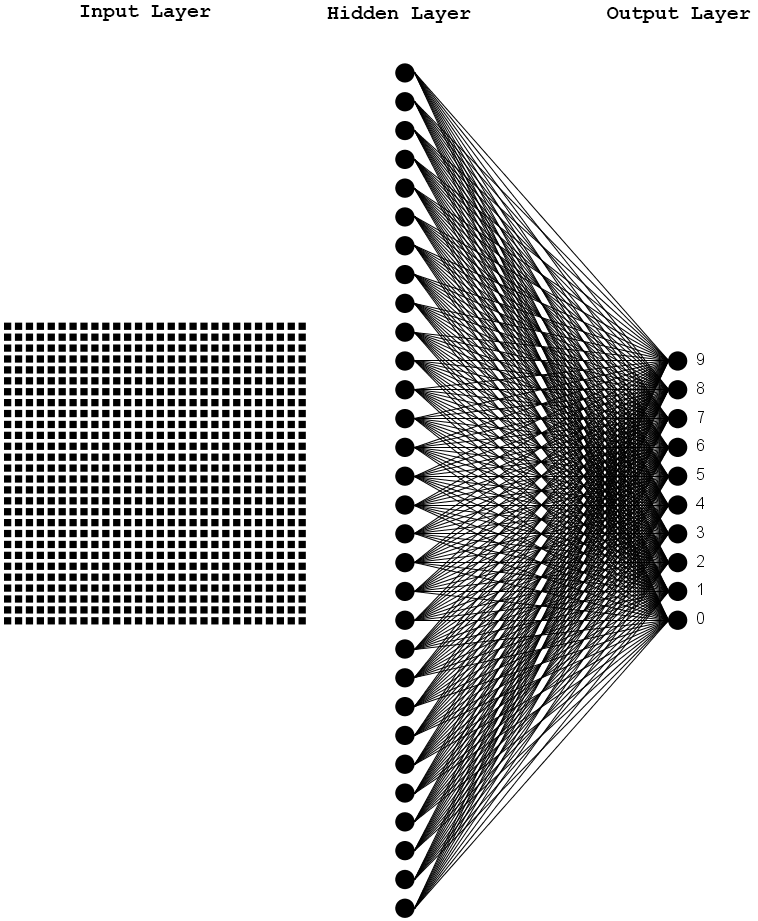
\includegraphics[scale=0.7]{Bilder/animation_network_default}
	\caption{Default Animation, welche über die Eingabe mit dem Wert $0$ aufgerufen wird.} 
	\label{fig:animation_network_default} 
\end{figure}
 
\noindent
Die \textbf{Eingabebefehle 1 - 30} betrachten den Untersuchungsbereich eines einzelnen Neurons der verborgenen Schicht, welches hierbei bei der Auswahl farblich hervorgehoben wird. Der Untersuchungsbereich ist farblich in rote und blaue Bereiche aufgeteilt. Pixel mit einer roten Färbung, haben eine hohe Gewichtung. Dahingegen weisen Pixel mit einer blauen Färbung einen geringen Gewichtungsfaktor auf. Blassere Farben haben hierbei eine geringere Merkmalsausprägung. Die Animation weist hierbei den folgenden Aufbau auf (siehe Abb. \ref{fig:untersuchungsbereich_neuron}).

\begin{figure}[!hbt]
	\centering
	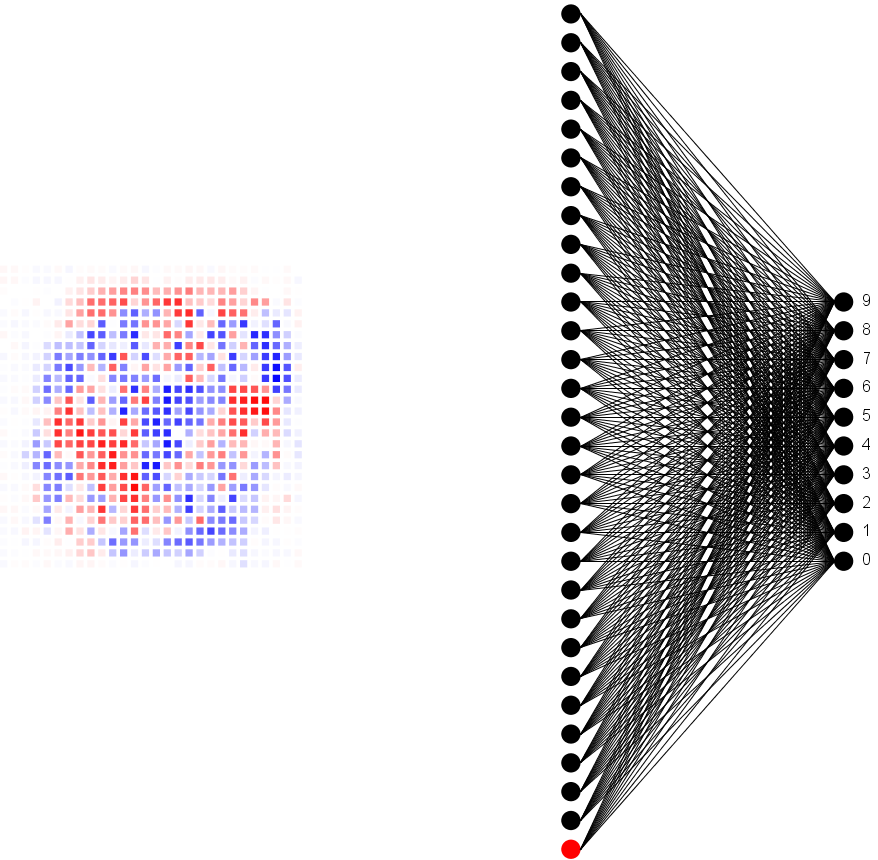
\includegraphics[scale=0.6]{Bilder/untersuchungsbereich_neuron}
	\caption{Untersuchungsbereich eines einzelnen Neurons der verborgenen Schicht.} 
	\label{fig:untersuchungsbereich_neuron} 
\end{figure}

\noindent
Über den \textbf{Eingabebefehl 1000} wird der Untersuchungsbereich von allen Neuronen in einer Übersicht abgebildet. Dies bedeutet, dass dieser Befehl die Ausgaben von den Eingabebefehlen 1-30 in sich zusammenfasst (siehe Abb. \ref{fig:untersuchungsbereich_neuronen}). Die grafische Ausgabe ermöglicht dem Anwender die Untersuchungsbereiche verschiedener Neuronen zu vergleichen und gegenüberzustellen. Konzentriert sich ein Neuron im Vergleich zu allen anderen nur auf einen bestimmten Bereich? Nimmt ein Neuron für die Erkennung einer handgeschrieben Zahl (z.B. $6$) einen größeren Einfluss wie andere Neuronen? \\

\begin{figure}[hbt]
	\centering
	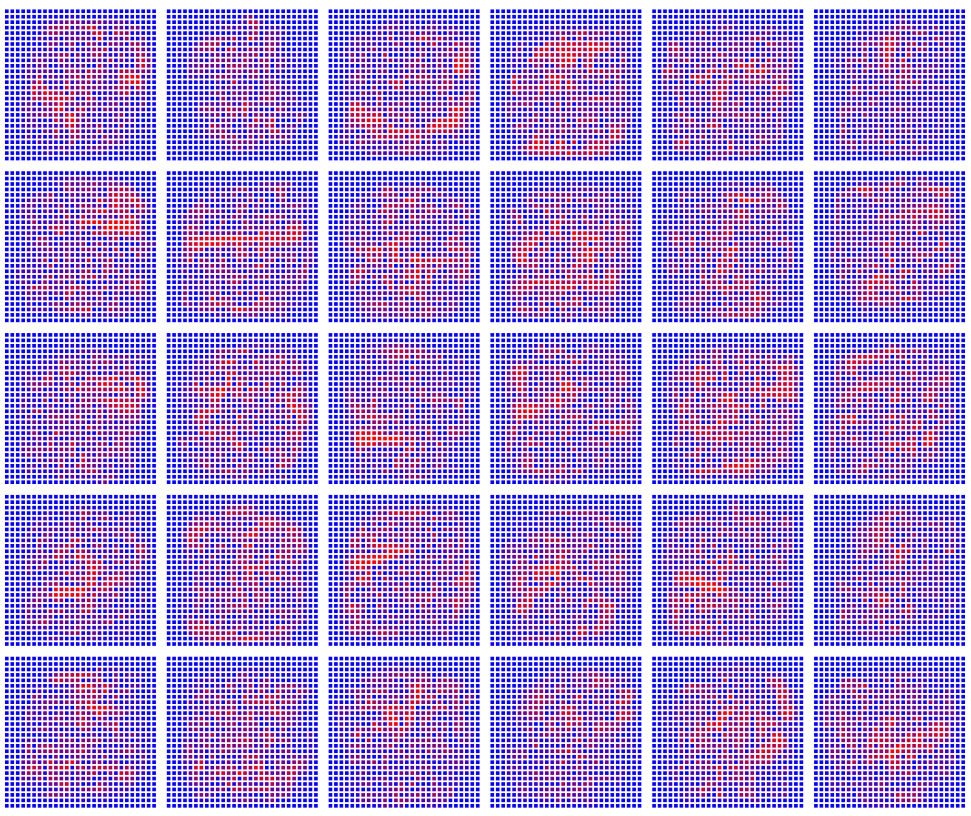
\includegraphics[scale=0.56]{Bilder/untersuchungsbereich_neuronen}
	\caption{Untersuchungsbereich aller Neuronen der verborgenen Schicht.} 
	\label{fig:untersuchungsbereich_neuronen} 
\end{figure}

\noindent
Der letzte \textbf{Eingabebereich 101-Datensatzgröße} ermöglicht den Untersuchungsbereich der Neuronen hinsichtlich einer Eingabe aus den Trainingsdaten zu betrachten. Die farbliche Bedeutung für den Untersuchungsbereich ist wie folgt definiert:
\begin{center}
\begin{tabular}{lp{6cm}}
\textbf{Farbe}   & \textbf{Erklärung} \\
\hline \\
blau, grün & Bereich mit einer geringen Relevanz \\[0.2cm]
rot, gelb  & Bereich mit einer hohen Relevanz   \\
\end{tabular}
\end{center}
Weiterhin ist wird das Untersuchungsobjekt, die Eingabe, sowie die Ausgabe mit dem berechneten Ergebnissen in der Animation abgebildet (siehe Abb. \ref{fig:untersuchungsbereich_zahl}). Die berechneten Ergebnisse ermöglichen dem Nutzer zu überprüfen, ob die Klassifizierung durch das neuronale Netzwerk richtig vorgenommen wurde und welche Neuronen in bei der Ergebnisfindung höheren Einfluss nehmen. Die Berechnung unter jedem Untersuchungsbereich ist durch die Sigmoid-Funktion bestimmt. \\

\noindent
An dieser Stelle soll angemerkt sein, dass aufgrund der Verwendung von nur einer verborgenen Schicht in diesem Versuchsaufbau und der Anzahl von nur 30 Iterationen keine Erkenntnisse anhand der grafischen Ausgaben getroffen werden können. Hierzu müsste ein \textit{Multilayer-Network} mit einer wesentlichen höheren Anzahl von Iterationen implementiert werden.

\begin{figure}[hbt]
	\centering
	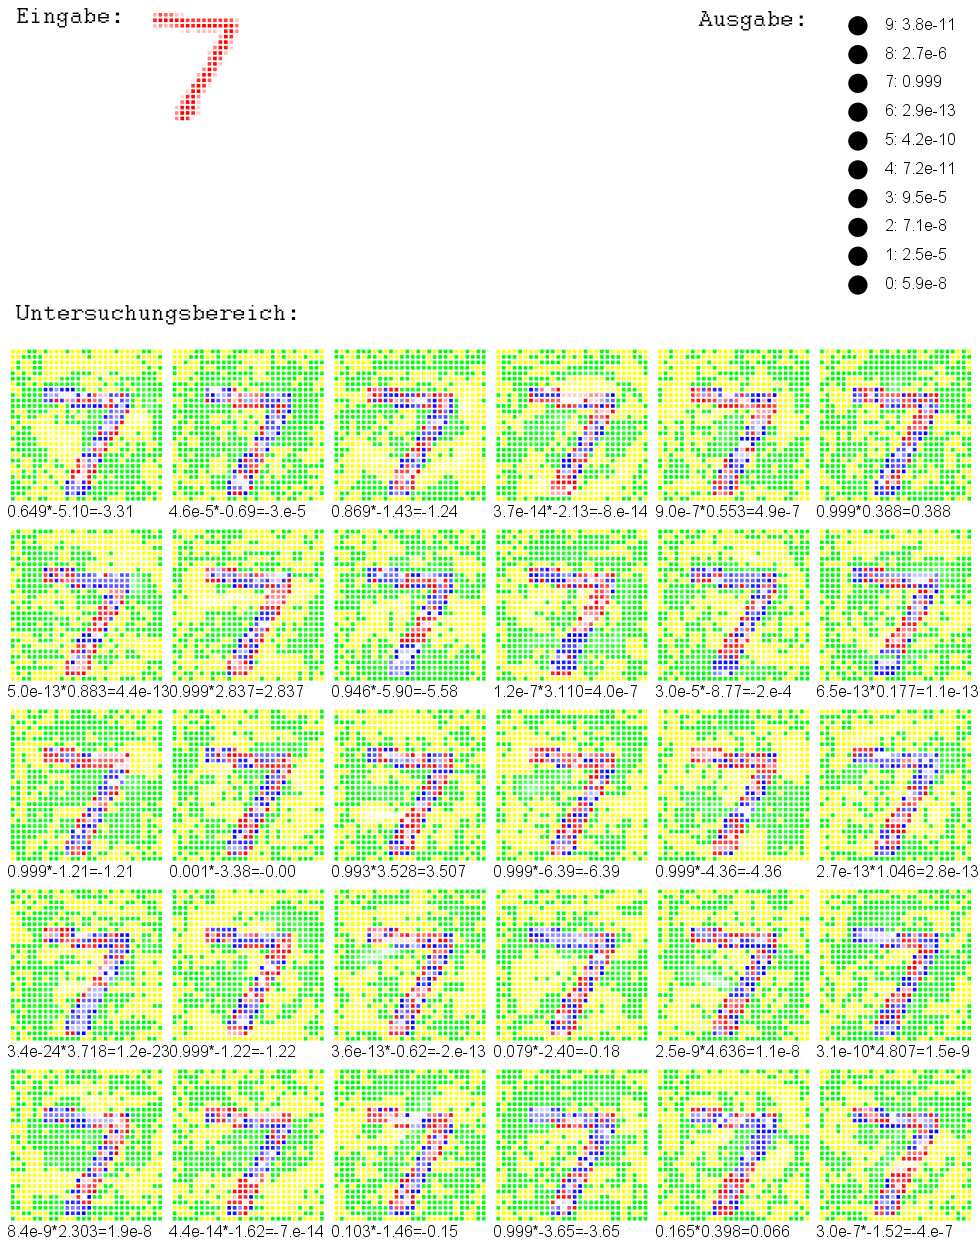
\includegraphics[scale=0.56]{Bilder/untersuchungsbereich_zahl}
	\caption{Untersuchungsbereich aller Neuronen der verborgenen Schicht hinsichtlich einer Eingabe.} 
	\label{fig:untersuchungsbereich_zahl} 
\end{figure}

\chapter{Fazit und Ausblick}

\section{Auswertung des Ergebnisses}
Die Umsetzung der Handschriftenerkennung von Ziffern mittels einem neuronalen Feedforward-Netz wurde erfolgreich in SetlX implementiert. Die Erkennungsrate des Netzwerkes liegt ungefähr zwischen 94 und 96 Prozent. Die nachfolgende Ausgabe in Abbildung \ref{fig:ausgabe_netzwerk} entspricht einem Durchlauf der $\mathtt{start.stlx}$-Datei. Hierbei wurden 10.000 Testdaten und 60.000 Trainingsdaten der MNIST-Datensätze verwendet. Die Epochenanzahl des Durchlaufs beträgt 30.

\begin{figure}
\begin{Verbatim}[ frame         = lines, 
                  framesep      = 0.3cm, 
                  firstnumber   = 1,
                  labelposition = bottomline,
                  numbers       = left,
                  numbersep     = -0.2cm,
                  xleftmargin   = 0.8cm,
                  xrightmargin  = 0.8cm,
                ]
    D:\DHBW\Neural-Network-in-SetlX\setlx>setlx start.stlx
    Reading file:   mnist_test.csv
    Image 10000 of 10000 imported
    End reading:    mnist_test.csv
    Reading file:   mnist_train.csv
    Image 10000 of 60000 imported
    Image 20000 of 60000 imported
    Image 30000 of 60000 imported
    Image 40000 of 60000 imported
    Image 50000 of 60000 imported
    Image 60000 of 60000 imported
    End reading:    mnist_train.csv
    Create Network
    Init Network
    Start SGD
    Epoch 1: 9427 / 10000
    Epoch 2: 9446 / 10000
    Epoch 3: 9534 / 10000
    Epoch 4: 9489 / 10000
    Epoch 5: 9581 / 10000
    Epoch 6: 9548 / 10000
    Epoch 7: 9559 / 10000
    Epoch 8: 9602 / 10000
    Epoch 9: 9543 / 10000
    Epoch 10: 9605 / 10000
    Epoch 11: 9571 / 10000
    Epoch 12: 9566 / 10000
    Epoch 13: 9603 / 10000
    Epoch 14: 9603 / 10000
    Epoch 15: 9598 / 10000
    Epoch 16: 9609 / 10000
    Epoch 17: 9587 / 10000
    Epoch 18: 9604 / 10000
    Epoch 19: 9609 / 10000
    Epoch 20: 9616 / 10000
    Epoch 21: 9591 / 10000
    Epoch 22: 9597 / 10000
    Epoch 23: 9605 / 10000
    Epoch 24: 9612 / 10000
    Epoch 25: 9588 / 10000
    Epoch 26: 9600 / 10000
    Epoch 27: 9598 / 10000
    Epoch 28: 9605 / 10000
    Epoch 29: 9582 / 10000
    Epoch 30: 9629 / 10000
    Time needed:    1255425ms		
\end{Verbatim}
\vspace*{-0.3cm}
\caption{Ausgabe des Netzwerkes}
\label{fig:ausgabe_netzwerk}
\end{figure}

\section{Performance der SetlX Implementierung}
Wie im vorherigen Kapitel zu sehen ist, beträgt die Durchlaufzeit des Programmes mit allen Datensätzen und 30 Epochen (Messzeit beginnt ab Aufruf der SGD-Funktion des Netzwerkes) 1255425 Millisekunden. Im Schnitt wurden ca. 1350000 Millisekunden benötigt, was 22,5 Minuten entspricht. Alle Messungen wurden auf einem Computer mit folgenden Hardwarekomponenten durchgeführt (nur relevante Komponenten sind aufgelistet):
\begin{itemize}
	\item \underline{CPU:} Intel Core i7-4720HQ @ 2.60GHz
	\item \underline{Arbeitsspeicher:} 16GB RAM
	\item \underline{Grafikkarte:} NVIDIA GeForce GTX 960M
\end{itemize}
% Alter Text:
% Python benötigte für den Durchlauf der 30 Epochen auf dem selben Computer ungefähr 210000 Millisekunden. Das sind im Durchschnitt 1140000 Millisekunden (19 Minuten) weniger als in der SetlX Implementierung.
Auffällig bei der Analyse der Laufzeit ist, dass die Durchlaufzeit der SetlX-Implementierung weit über der der Python-Implementierung liegt. SetlX benötigte für den Durchlauf der 30 Epochen auf dem selben Computer im Schnitt 5,4 mal länger als die Python-Version des Programms. Basierend auf einer Reihe Performance-Tests, die auf Grund der langen Durchlaufzeiten durchgeführt wurden, stellte sich heraus, dass die Matrizen-Multiplikation in SetlX wesentlich zeitintensiver ist als in der Numpy-Bibliothek von Python. Der Faktor hierbei beträgt circa 6,5. \\
Eine Vermutung, wieso die SetlX Matrizen-Multiplikation wesentlich langsamer ist, ist dass in Python die Berechnung auf die Grafikkarte des Computers ausgelagert wird. Da die Programmiersprache Java (welche die Grundlage von SetlX bildet) plattformunabhängigkeit verspricht, wäre es möglich, dass hier keine Auslagerung auf die Grafikkarte stattfindet. Allerdings sind dies nur erste Vermutungen und müssten auf Ebene der JAMA-Bibliothek (wird von SetlX zur Matrizen-Multiplikation verwendet) in Java, sowie der Numpy-Bibliothek in Python überprüft werden. \\ \\
Die gesamte Auswertung sowie alle hierfür verwendeten Programme sind im Verzeichnis
\\[0.2cm]
\hspace*{1.3cm}
/setlx/testing/
\\[0.2cm]
im GitHub-Repository zu finden. Die Datei $\mathtt{setlx\_performance\_evaluation.pdf}$ bietet eine Übersicht und Beschreibungen zu den durchgeführten Tests.

%\bibliographystyle{alpha}
\bibliography{cs}
%\bibliography{/Users/stroetma/Dropbox/Kurse/cs}

\end{document}



